\documentclass[12pt]{report}
\usepackage[a4paper]{geometry}
\usepackage{slovak}
\usepackage{epsfig}
\usepackage{color}
\usepackage{url}
\usepackage[utf8]{inputenc}
\usepackage{amsmath}
\usepackage{amsfonts}
\usepackage{amssymb}
\usepackage{mathtools}
\usepackage{listings}
\usepackage{algpseudocode}
\usepackage{algorithm}
\usepackage{program}
\usepackage{multicol}
\usepackage{framed}
\usepackage{titlesec}

\definecolor{gray}{rgb}{0.4,0.4,0.4}
\definecolor{darkblue}{rgb}{0.0,0.0,0.6}
\definecolor{cyan}{rgb}{0.0,0.6,0.6}

\lstset{
  basicstyle=\ttfamily,
  columns=fullflexible,
  showstringspaces=false,
  commentstyle=\color{gray}\upshape
}

\lstdefinelanguage{XML}
{
  morestring=[b]",
  morestring=[s]{>}{<},
  morecomment=[s]{<?}{?>},
  stringstyle=\color{black},
  identifierstyle=\color{darkblue},
  keywordstyle=\color{cyan},
  morekeywords={xmlns,version,type}% list your attributes here
}

\lstset{language=XML}

\renewcommand\baselinestretch{1.5} % riadkovanie jeden a pol 1.3

% pekne pokope definujeme potrebne udaje
\def\mftitle{Editor voxelovej grafiky}
\def\mfthesistype{Bakalárska práca}
\def\mfauthor{Marek Kružliak}
\def\mfadvisor{RNDr. Martin Samuelčík, PhD.}
\def\mfplacedate{Bratislava, 2013}
\def\mfprogram{Aplikovaná informatika}

\ifx\pdfoutput\undefined\relax\else\pdfinfo{ /Title (\mftitle) /Author (\mfauthor) /Creator (PDFLaTeX) } \fi

\begin{document}

% obal
\begin{titlepage}
	\begin{minipage}{0.2\textwidth}
	
\includegraphics[width=0.9\textwidth]{komlogo-new.pdf}
	\end{minipage}
	\begin{minipage}{0.8\textwidth}
	\begin{center}
		\sc
		Univerzita Komenského, Bratislava \\
		Fakulta Matematiky, Fyziky a Informatiky 
	\end{center}
	\end{minipage}
	
	\vspace*{\fill}
	\begin{center}
	{\LARGE\sc\mftitle} \\
	\smallskip	
	\mfthesistype
	\end{center}
	\vspace*{\fill}
	
	
	\begin{figure}[!h]
		\smallskip
		\smallskip
		\textbf{\mfplacedate} \\
		\hspace{1pt} \textbf{\mfauthor}
	\end{figure}
\end{titlepage}
% titulna strana
\begin{titlepage}
	\begin{minipage}{0.2\textwidth}
	
\includegraphics[width=0.9\textwidth]{komlogo-new.pdf}
	\end{minipage}
	\begin{minipage}{0.8\textwidth}
	\begin{center}
		\sc
		Univerzita Komenského, Bratislava \\
		Fakulta Matematiky, Fyziky a Informatiky 
	\end{center}
	\end{minipage}
	
	\vspace*{\fill}
	\begin{center}
	{\LARGE\sc\mftitle} \\
	\smallskip	
	\mfthesistype
	\end{center}
	\vspace*{\fill}
	
	\begin{figure}[!h]
		\bigskip
		\bigskip
		\begin{minipage}[h]{0.3\textwidth}
		  Študijný program: 	    \\
		  Študijný odbor:			\\
		  Školiace pracovisko: 	\\
		  Školiteľ: 				
		\end{minipage}
		\begin{minipage}[h]{0.5\textwidth}
		  Aplikovaná informatika 	    \\
		  2511 Aplikovaná informatika 	    \\
		  Katedra aplikovanej informatiky 	    \\
		  \mfadvisor 	    
		  \end{minipage}
	\end{figure}
	
	\begin{figure}
		\smallskip
		\smallskip
		\textbf{\mfplacedate} \\
		\hspace{1pt} \textbf{\mfauthor}
	\end{figure}
\end{titlepage}
% Zadanie
\newgeometry{top=0.3cm, bottom=0.0cm}
\thispagestyle{empty}
\noindent\makebox[\textwidth]{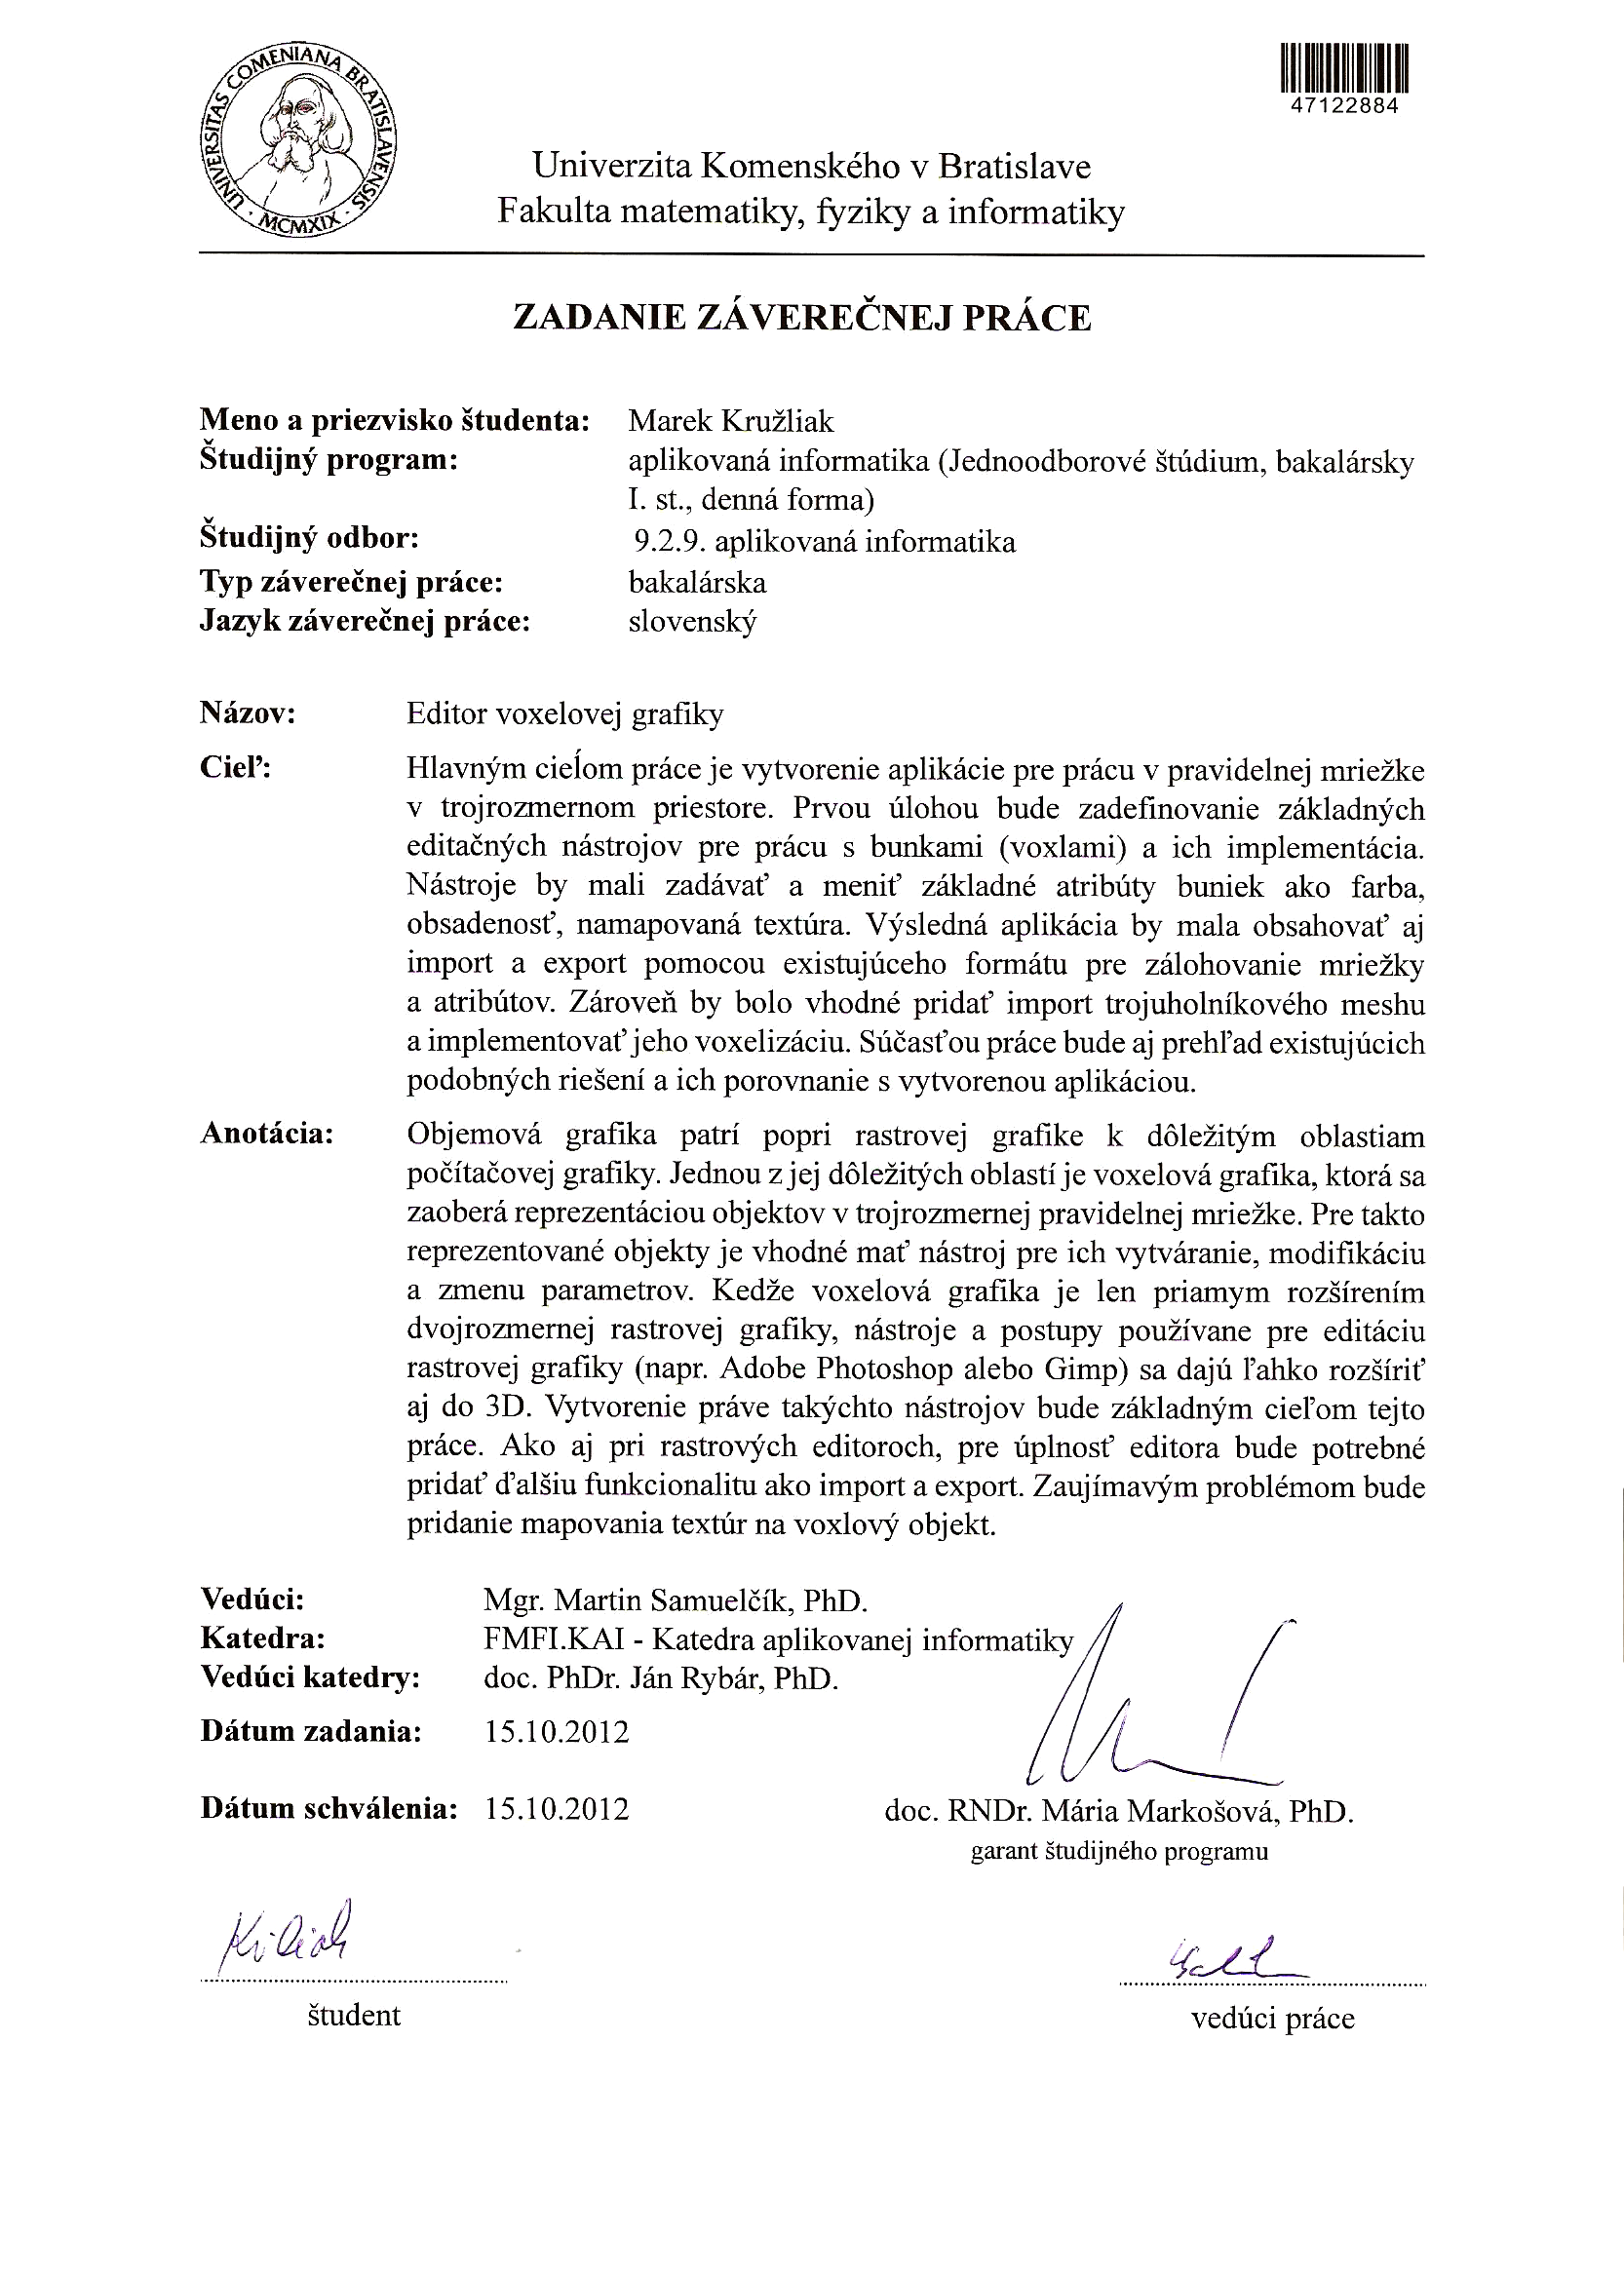
\includegraphics[width=597pt,height=845pt,keepaspectratio]{zadanie.png}}
\restoregeometry
%prehlasenie
\thispagestyle{empty}
\vspace*{\fill}
\hfill
\begin{minipage}{0.63\textwidth}
Čestne prehlasujem, že som túto bakalársku prácu vypracoval samostatne s použitím citovaných zdrojov.

\bigskip
	\begin{flushright}
	\begin{minipage}{0.5\textwidth}
	\dotfill
	\end{minipage}
	\end{flushright}
\end{minipage}\eject
% Podakovanie
\thispagestyle{empty}
\topskip0pt
\vspace*{\fill}
\hfill
\begin{minipage}{0.65\textwidth}
\vspace{0pt}\raggedright
Ďakujem RNDr. Martinovi Samuelčíkovi, PhD. za to, že sa
ujal vedenia mojej bakalárskej práce a za jeho cenné rady
pri programovaní a pri písaní práce. 
\end{minipage}
\vspace*{\fill}
\eject

\setcounter{page}{1}
\pagenumbering{Roman}
% abstrakt
\begin{Huge}
\textbf{Abstrakt}  \\
\end{Huge}

Primárnym cieľom práce je opísať návrh a implementáciu praktického nástroja na tvorbu 
a editovanie voxelových objektov a scén. 
V práci sa taktiež venujeme vysvetleniu základných pojmov objemovej grafiky a jej využitiu mimo vedeckej sféry, teda v moderných herných enginoch a podobne.
Ďalej uvádzame príklady existujúcich riešení v danej oblasti, ich kladné a záporné stránky, a následné
využitie získaných poznatkov z ich testovania.
Práca taktiež opisuje zaujímavé algoritmické problémy, ktoré sa počas tvorby práce vyskytli, ich riešenie a implementáciu opísaného riešenia.\\



\textbf{Kľúčové slová:} voxel , objemová grafika, voxelizácia
\eject

\begin{Huge}
\textbf{Abstract}  \\
\end{Huge}

Primary goal of this paper is to describe design and implmentation of voxel editing tool. We also describe basic concept of volume graphics and its usage in commercial sphere, like modern game engines, animation etc. Next we mention examples of already existing solutions in this field, their strong and weak points and their influence on this work. In this paper we also analyze intersesting algorithmic problems, which appeard during implementation phase. \\

\textbf{Keywords:} voxel, volume graphics, voxelization
\tableofcontents
%zoznam obrazkov a tabuliek
\listoffigures
\begingroup
\let\clearpage\relax
\listoftables
\endgroup
%zoznam skratiek
\eject
\begin{Huge}
\noindent\textbf{Zoznam skratiek} 
\end{Huge}


\begin{figure}[!h]
		\bigskip
		\bigskip
		\hspace{0.5cm}
		\begin{minipage}[h]{0.1\textwidth}
		  WRF \\
		  NCEP \\
		  NCAR \\
		  NWP \\
		  GFS \\
		  NAM \\
		  RUC \\
		  SREF \\
		  GEFS \\
		  ECMWF \\
		  NOAA \\
		  ESRL \\
		  AFWA \\
		  NRL \\
		  CAPS \\
		  LES \\
		  WMO \\
		  TOGA \\
		  ME \\
		  MFE \\
		  MAE \\
		  RMSE \\
		  MSE \\
		  TS \\
		  MAD \\
		  GUI \\
		  VBA \\
		  SAS \\
		  CAWCR \\
		  IDL \\
		  NCL \\
		  MET \\
		  DTC \\
		  EVS \\
		  HEP \\
		  MISE \\
		  KDE \\
		  IMS \\
		  HTML \\
		  SVG \\
		\end{minipage}
		\begin{minipage}[h]{0.8\textwidth}
		  Weather Research and Forecasting \\
		  National Centers for Environmental Prediction \\
		  National Center for Atmospheric Research \\
		  Numerical Weather Prediction \\
		  Global Forecast System \\
		  North American Mesoscale Forecast System \\
		  Rapid Update Cycle \\
		  Short Range Ensemble Forecast \\
		  Global Ensemble Forecast System \\
		  European Centre for Medium-Range Weather Forecasts \\
		  National Oceanic and Atmospheric Administration \\
		  Earth System Research Laboratory \\
		  Air Force Weather Agency \\
		  Naval Research Laboratory \\
		  The Center for Analysis and Prediction of Storms \\
		  Large eddy simulation \\
		  World Meteorological Organization \\
		  Tropical Ocean Global Atmosphere \\
		  Mean Error \\
		  Mean Forecast Error \\
		  Mean Absolute Error \\
		  Root Mean Square Error \\
		  Mean Square Error \\
		  Tracking Signal \\
		  Median Absolute Deviation \\
		  Graphical User Interface \\
		  Visual Basic for Applications \\
		  Statistical Analysis Software \\
		  Centre for Australian Weather and Climate Research \\
		  Interactive Data Language \\
		  NCAR Command Language \\
		  Model Evaluation Tools \\
		  Developmental Testbed Center \\
		  Ensemble Verification System \\
		  Hydrological Ensemble Prediction \\
		  Mean Integrated Square Error \\
		  Kernel Density Estimation \\
		  Integrated Monitoring System \\
		  Hypertext Markup Language \\
		  Scalable Vector Graphics \\
		  \end{minipage}
	\end{figure}
	
\begin{figure}[!h]
		\bigskip
		\bigskip
		\hspace{0.5cm}
		\begin{minipage}[h]{0.1\textwidth}
		  CSS \\
		  CSV \\
		  UML \\
		\end{minipage}
		\begin{minipage}[h]{0.8\textwidth}
		  Cascading Style Sheets \\
		  Comma Separated Values \\
		  Unified Modeling Language \\		 
		\end{minipage}
	\end{figure}	
	 
			  
			  
			  

\eject
\setcounter{page}{1} 
\pagenumbering{arabic}

\chapter{Úvod}
	
	
Vizualizácia informácií a vizuálna analýza dát sú dnes veľmi vyvíjaným a moderným odvetvím počítačovej grafiky. Aplikácie vizualizácie informácií sú rôzne od ... cez ... až po ... Úlohou vizualizácie informácií je v prvom rade využitie ľudských kognitívnych schopností pre lepšie porozumenie dát.

Svoje využitie našla aj v procese verifikácie predpovedných modelov počasia. Dnešné metódy verifikácie predpovedí sa sústreďujú na numerický popis výkonu jednotlivých predpovedných modelov pomocou rôznorodých štatistických metód. Vo výsledku sa dáta opisujú ďalšími dátami, avšak práve na vizualizáciu týchto dát sa kladie veľmi slabý dôraz.

V našej práci sme preštudovali používané štatistické metódy pre verifikáciu spojitých premenných, ktoré predpovedá model \textit{WRF}. Hlavným cieľom práce sa však stal návrh a implementácia vizualizačných techník špeciálne navrhnutých pre potreby verifikácie. Sústredili sme sa obzvlášť na to, aby sme ušetrili cenný vizuálny priestor bez straty potrebných informácií. Návrh vizualizácie vychádza ...
\chapter{Objemová grafika}\label{chap:grafika}
Vďaka pokroku vo vývoji hardvéru sa revolučné prístupy k počítačovej grafike postupne stávajú realitou, a to aj pre bežného majiteľa počítača. Dobrým ilustratívnym príkladom pre nás môže byť rastrová grafika, ktorá sa objavila v období, kedy hardvérové inovácie dopomohli k reálnemu presunu z matematicky reprezantovanej vektorovej grafiky k pamäťovo náročnejšej rastrovej grafike.
Podobným príkladom je aj objemová grafika, ktorej rozvoj opísali vo svojom článku v roku 1993
Kaufman, Cohen a Yagel \cite{VolumeGraphics}.

Objemová grafika teda predstavuje prechod od takzvanej povrchovej grafiky, ktorá objekty reprezentuje pomocou spojitých primitív ako sú polygóny alebo free-form povrchy, k reprezentácii objektu pomocou diskrétnych objemových štruktúr \cite{Winter}, ktorých základná dátová jednotka je voxel opísaná nižšie v tejto kapitole.
Taktiež môžme povedať, že objemová grafika je významným poľom počítačovej grafiky a je 3D analógiou rastrovej grafiky. Jej uplatnenie sa našlo nielen vo vizualizácii rôznorodých vedeckých dát, ale aj v komerčnom využití ako napríklad herné enginy, animácie alebo umenie.

Avšak objemová grafika naďalej zostáva menšinou na poli počítačovej grafiky, pretože jednou z hlavných prekážok jej širšieho použitia je fakt, že niektoré z fundamentálnych operácií ešte potrebujú vylepšenie teoretických základov a taktiež objemová grafika, na rozdiel od tej povrchovej, nemá podporu grafických akcelerátorov. Na druhej strane sa mnohé z techník objemovej grafiky stali populárnymi v radoch
vývojárov najrôznejších grafických aplikácií, pretože objavili nesporné výhody tohto
prístupu v určitých oblastiach.
\cite{Tomas}

\section{Objemové dáta}
Ako bolo spomenuté vyššie, najbežnejším prístupom k reprezantácii objektov v trojrozmernom priestore je
povrchová reprezentácia objektov pomocou dvojrozmerných primitív. Tento prístup je však v mnohých prípadoch nedostačujúci, pretože sa takto strácajú informácie o vnútornej štruktúre 3D telies.
Nastolený problém riešia objemové dáta, ktoré tieto informácie obsahujú. Vďaka tejto vlastnosti je objemová reprezentácia vhodný kandidát pre medicínske, geologické, biologické, archeologické a iné vedecké dáta získané napríklad v prípade medicíny z tomografu.\cite{RealTime} V hernom priemysle je takáto reprezentácia vhodná na detajlnú deštrukciu okolitého prostredia alebo je taktiež vhodná na modelovanie amorfných objektov ako sú napríklad oblaky, dym a podobne. 

Vizualizácia objemových dát sa markantne líši od vizualizácie povrchových telies, keďže objemové dáta neobsahujú žiadnu explicitnú ifnormáciu o povrchu a taktiež je nevyhnutne potrebné nejako nahliadnuť do vnútra objektu. Cieľom vizualizácie objemových dát je teda vytvoriť mechanizmus, ktorý nám umožní extrahovať zmysluplné infromácie z objemových dát pomocou ich reprezentácie, manipulácie a renderingu.

Objemové dáta sa najčastejšie uchovávajú v trojrozmernom poli a teda sú zvyčajne reprezentované ako štvorica $(x,y,z,v)$, kde $(x,y,z)$ sú poloha v 3D priestore $v$ je $value$, teda hodnota danej objemovej jednotky, čo môže byť napríklad $0$ alebo $1$, kde hodnota $0$ indikuje prázdne miesto a $1$ indikuje objekt. Táto hodnota môže byť aj komplexnejšia informácia, ako napríklad farba, hustota, tlak alebo vektor zrýchlenia v danej polohe $(x,y,z)$.
\cite{VolumeGraphics} Alternatívne dátové štruktúry na uchovávanie a manipuláciu objemových dát sú napríklad octrees, voxelové riedke matice, '\textit{voxel runs}' alebo nepravideľné mriežky. Tieto štruktúry sú zvyčajne vhodné na dobrý manažment pamäťových zdrojov alebo majú iné výhody napríklad v detekcii kolízií.
\section{Voxel}
Elementárnou jednotkou objemovej grafiky je voxel. Je priamou 3D analógiou pre jednotku dvojrozmerného priestoru v pravidelnej mriežke, teda pixel. Podobne ako slovo pixel (picture element) slovo voxel je len skratkou pre zložitejšie pomenovanie volume element. Ako bolo dostatočne opísané v predchádzajúcej kapitole, každý voxel okrem svojej polohy v priestore obsahuje aj nejakú merateľnú hodnotu. 

Analógia, pre voxeli s pixelmi, sa zachováva aj pri uchovávaní voxelov v pravidelnej mriežke. Teda zatiaľ čo sú pixely uchovávané vo \textit{frame buffery}, voxely sa uchovávajú vo \textit{volume buffery} alebo tiež nazývanom \textit{3D raster}, či \textit{objemový frame buffer}.

Zadefinovaním tohto pojmu môžeme teraz hovoriť o voxelovom priestore alebo tiež o voxelovej grafike.

\section{Porovnanie s povrchovou grafikou}
Spomenuli sme už majoritné rozdiely medzi povrchovou a voxelovou grafikou, ktoré priamo vyplývajú z ich pomenovania. V tejto časti sa teda zameriam na porovnanie týchto dvoch prístupov detajlnejšie s dôrazom na výhody a nevýhody objemovej grafiky oproti povrchovej.

\subsection{Nevýhody}
Pri reprezentácii scény sú voxely usporiadané v pravidelnej trojrozmernej mriežke, teda hovoríme o diskrétnom priestore. Tento fakt spôsobuje mnohé komplikácie analogické ku komplikáciám v rastrovej grafike.

Jedným z hlavných problémov je poškodenie, teda modifikácia alebo strata informácii o objekte pri jeho transformácii. Pri rotácii objektu o uhol \begin{math} \alpha \neq k\frac{\pi}{2}, k \in \mathbb{Z} \end{math}  vznikajú diery. Podobne aj pri škálovaní o koeficient \begin{math}k > 1\end{math} je očakávaný vznik dier a pri škálovaní o koeficient \begin{math}k < 1\end{math} nastáva strata informácie. Keďže tieto problémy súvisia taktiež s rastrovou grafikou, vzniklo dostačujúce množstvo techník (supersampling, bilineárna interpolácia a pod.) ako tento problém riešiť s viac-menej uspokojivým výsledkom.

Keďže voxelové objekty sú získavané vzorkovaním, nevyhnutne vznikajú artefakty. Tie vidieť najmä pri bližšom zazoomovani na danú oblasť. Teda môžme povedať, že voxelové objekty sú nepresné a sú len diskrétnou aproximáciou pôvodných objektov, kde hustota 3D mriežky určuje ich presnosť.

Prítomnosť objemu vo voxelových objektoch spôsobuje ďalší problém charakteristický pre voxelovú grafiku, a tým je pamäťová a procesová náročnosť. Pomerne malý objekt s rozmermi \begin{math}512^{3}\end{math} pozostáva z približne \begin{math}1.35\cdot 10^{8}\end{math} voxelov. Ak by sme každý voxel reprezentovali iba jediným bytom, tak pre takýto objekt by bolo potrebné 128MB pmäte. Tieto veľké objemy priamo spôsobujú, že voxelová grafika je náročná aj na processing. Príkladom môže byť rendering, transformácie alebo aj voxelizácia.

\subsection{Výhody}
Okrem niekoľkokrát spomenutého faktu, že objemová grafika obsahuje aj informácie o vnútornej štruktúre objektov, nám voxelový priestor ponúka ďalšie nesporné benefity.

Jedným z nich je jednoduchosť rôznych operácií, ako je napríklad sekanie, orezávanie alebo aj booleanovské operácie medzi objektami. Zatiaľ čo pri povrchovej grafike sú tieto operácie pomerne komplexné a zložito implementovateľné, vo voxelovej grafike sa tieto operácie posúvajú až na úroveň voxelov a teda predstavujú triviálny problém. Ak si zvolíme Constructive Solid Geometry (CSG) ako modelovaciu paradigmu, tak je táto vlastnosť voxelových objektov ohromnou výhodou.

Ďalšou výhodou je, že voxelová grafika nie je citlivá na členitosť objektov. Pri väčšej členitosti objektu v povrchovej grafike narastá počet polygónov a teda aj požiadavky na zdroje, zatiaľ čo voxelový objekt si svoju zložitosť zachováva konštantnú. Podobne aj pri mapovaní textúr (znázornené na obrázku \ref{tank}) má objemová grafika výhodu, pretože na voxelový objekt stačí namapovať textúru iba raz, kedy sa vypočíta farba pre každý voxel a v ňom sa aj naďalej uchováva, zatial čo mapovanie textúr na polygónový respektíve povrchový objekt sa vykonáva zvyčajne až na konci renderovacej pipeline.

\begin{figure}[ht!]
	\centering
	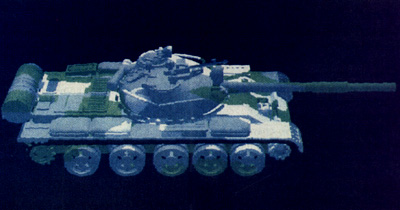
\includegraphics[width=90mm]{tank.jpg}
	\caption[Voxelový tank s namapovanou textúrou]{Voxelový tank s namapovanou textúrou}
	\label{tank}
\end{figure}

\eject

\section{Komerčné využitie}
Technologický pokrok umožnil, že objemovú grafiku je možné realizovať aj na bežnom-širokodostupnom hardvéri. Toto otvorilo dvierka pre komerčnú sféru technologického rozvoja, a tak sa voxely objavujú nielen ako pomôcka pre zobrazenie pseudonáhodných čísel v teoretickej informatike, ale aj ako stavebné častice herného prostredia, či nástroj na tvorbu detajlných skulptúr.

\subsection{Herný priemysel}
Prvou firmou, ktorá sa odvážila využiť voxely ako stavebný prvok pre svoj herný engine bola spoločnosť \textit{NovaLogic} v roku 1992 v hre \textit{Comanche: Maximum Overkill} \cite{VoxelGames} . Išlo o letecký simulátor, ktorý voxelovú technológiu použil na vytvorenie detajlného vykreslenia okolitého terénu, aký je na obrázku \ref{comanche}. V roku 1996 táto spoločnosť za podobným účelom vytvorila populárnu bojovú hru \textit{Delta Force}.

V roku 2000 začal pracovať programátor Ken Silverman spolu s Tomom Dobrowolskym na svojom prvom plne voxelovom hernom engine s názvom \textit{Voxlap}. \cite{Voxlap} Ten je teraz spolu so zdrojovými kódmi voľne dostupný na svojej oficiálnej stránke a ponúka vykreslovanie voxelového priestoru v pomerne dobrom rozlíšení.

Hra, ktorá najviac spopularizovala voxelovú grafiku vo svojej upravenej podobe, vznikla v roku 2010 s názvom \textit{Minecraft}. Princípom hry je dolovať v hlbokom podzemí bloky rôznych stavebných materálov. Takýmto spôsobom hra využíva najdôležitejšiu vlastnosť voxelovej grafiky, ktorou je uchovanie infromácie o vnútornom obsahu objektu. 

\begin{figure}[ht!]
	\centering
	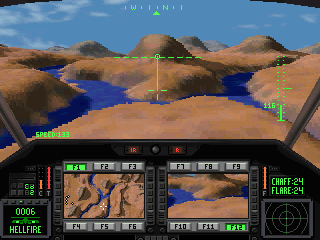
\includegraphics[width=90mm]{comanche.png}
	\caption[Ukážka voxelového terénu z hry Comanche: Maximum Overkill]{Ukážka voxelového terénu z hry \textit{Comanche: Maximum Overkill}}
	\label{comanche}
\end{figure}

\subsection{Umenie}
Informatika a obzvlášť počítačová grafika je natoľko ohromujúca, že svojím vplyvom zasahuje i do umenia. Nie je teda prekvapením, že voxely si našli svoje miesto aj medzi umelcami. 

Dobrým príkladom je napríklad aj digitálne sochárstvo (\textit{Voxel sculpting}). To umožňuje pre umelca slobodu modelovania digitálnych sôch bez akýchkoľvek topologických obmedzení a vytvárať komplexné detajly takmer z ničoho. Táto sloboda je dosiahnutá vďaka tomu, že úprava sôch nie je založená na deformácii povrchu, ale na vytváraní a vyplňovaní objemu. \cite{Sculpting}

Voxelart je ďalším smerom digitálneho umenia, ktoré je 3D obnožou pre pixelart. Na rozdiel od digitálneho sochárstva vo voxelarte sa kladie dôraz na každý vložený voxel, ktorý dotvára celkový dojem z diela. Zvyčajne takéto výtvory bývajú aj omnoho jednoduchšie, keďže ich tvorba je náročnejšia.

Svojou jedinečnosťou zaujali voxely aj animátorov a na internete je možnosť nájsť pomerne veľké množstvo zaujímavých kockatých animácií.
\chapter{Existujúce riešenia}\label{chap:riesenia}
Napriek vzrastajúcej popularite voxelovej grafiky neexistuje doposiaľ mnoho kvalitných nástrojov na ich editáciu. Preto sme vybrali niektoré z nich, ktoré nám svojim charakterom najviac vyhovujú. 
Celkovo môžme rozdeliť takéto programy do dvoch skupín. Jednou sú programy slúžiace na digitálne sochárstvo s voxelovým základom a druhou sú nástroje zámerne zobrazujúce každý voxel.

\section{Digitálne sochárstvo}
Digitálne sochárstvo je pomerne nová a zaujímavá metóda 3D modelovania. Umožňuje pridávanie najjemnejších detajlov a v prípade voxelových programov aj bez ohľadu na topológiu modelu. Vďaka tomu aj napriek pomerne krátkej existencii sa táto metóda stala veľmi populárnou medzi tvorcami detajlnej 3D grafiky. Voxelové sochárstvo sa prevažne využíva na tvorbu modelov s fotorealistickým až hyperrealistickým vzhľadom, ktoré slúžia ako predlohy do filmov, hier, priemyselného dizajnu a taktiež ako realistické ilustrácie a podobne. Nechceme sa však zamerať na tento smer modelovania, keďže nevyužíva voxely ako základnú stavebnú jednotku, ale len ako nástroj k zlepšeniu detajlov modelov alebo ako nástroj umožňujúci slobodnejšiu tvorbu.

Zoznam zaujímavých voxel-based programov pre digitálne sochárstvo:
\begin{itemize}
	\item \textbf{3Dcoat} Program, ktorý zadefinoval pojem \textit{Voxel Sculpting}.
	\item \textbf{Acropora} Procedurálny voxelový modeler.
	\item \textbf{Crysis Terrain editor} Program na tvorbu členitých terénov do počítačovej hry \textit{Crysis}.
\end{itemize}

\section{Editory voxelovej grafiky}
V tejto časti sa zameriavame na programy, ktoré na rozdiel od nástrojov na digitálne sochárstvo nevyužívajú voxely len ako pomôcku k dosiahnutiu detajlného výsledku s pomerne vysokým levelom slobody tvorby, ale ako primárnu stavebnú jednotku 3D objektov. Takéto nástroje neumožňujú veľké rozlíšenia voxelových priestorov a teda nie sú ani zamerané na detajl modelov. Toto spôsobuje, že užívateľ má pod kontrolou každý voxel scény, ale aj to, že sú viditeľné rôzne artefakty, obzvlášť zubatý okraj objektov. Takýto stav nemožno nazvať nevýhodou, keďže mnoho fanúšikov voxelov ostré hrany obľubuje, pretože práve viditeľné kocky dodávajú voxelovej grafike to správne čaro.

Nasledujúci prehľad obsahuje vzorku voxelových editorov, ktoré sa nám podarilo nainštalovať a korektne spustiť. Taktiež obsahuje ich stručný opis s výhodami a nevýhodami, ktoré sme zaznamenali pri krátkom testovaní.
\subsection{Paint3D}
Daný program predstavuje jednoduchú 3D alternatívu pre program MS Paint \cite{paint3d}. Interface aplikácie je zobrazený na obrázku \ref{obr:paint3D}.
\subsubsection{Výhody:}
\begin{itemize}
	\item \textbf{Jednoduchosť}. Na webovej stránke tohoto programu tvorcovia proklamujú, že je nástroj jednoduchý na používanie. Do istej miery je to aj pravda, avšak pri testovaní sme museli využiť niektoré internetové zdroje, aby sme pochopili, ako program funguje. 
	\item \textbf{Nástroje}. V ponuke sú rôzne užitočné nástroje a je ich taktiež primerané množstvo.
	\item \textbf{Priehladnosť}. Program podporuje, ako jediný z testovaných, alfa transparenciu voxelov.
	\item \textbf{Spolupráca sa 2D grafickými programami}. Tento nástroj umožňuje funkcie copy/paste z iných 2D grafických programov, ako je napríklad MS Paint od spoločnosti \textit{Microsoft}.
	\item \textbf{Kresliace módy}. Program ponúka viaceré módy kreslenia voxelov. Či už po rezoch v rôznych osiach alebo priestorovým kreslením štetcom s nastaviteľnou hrúbkou.
	\item \textbf{Export/Import}. Program podporuje široké množstvo voxelových formátov.
	\item \textbf{Skriptovanie}. Asi najväčšou výhodou tohto nástroja je skriptovanie, ktoré sa dá v grafike a vo voxelovej obzvlášť dobre využiť pri tvorbe inak pracne vytvorených modelov.  
\end{itemize}

\subsubsection{Nevýhody:}
\begin{itemize}
	\item \textbf{Zahlcovanie procesora}. Program už pri spustení a počas celého behu vyťaží procesor na takmer 100\%. Toto by nemal robiť žiaden rozumný program pri pokojovom stave.
	\item \textbf{Plná verzia je platená}. Ak by ste chceli využívať všetky možnosti programu, musíte si priplatiť 20\$. Našťastie je trial verzia voľne stiahnuteľná a to, čo ponúka je dostačujúce na prácu.
	\item \textbf{Jeden objekt v scéne.} Možnosť pridávania viacerých objektov do scény neumožňuje väčšina programov.
\end{itemize}
\begin{figure}[ht!]
	\centering
	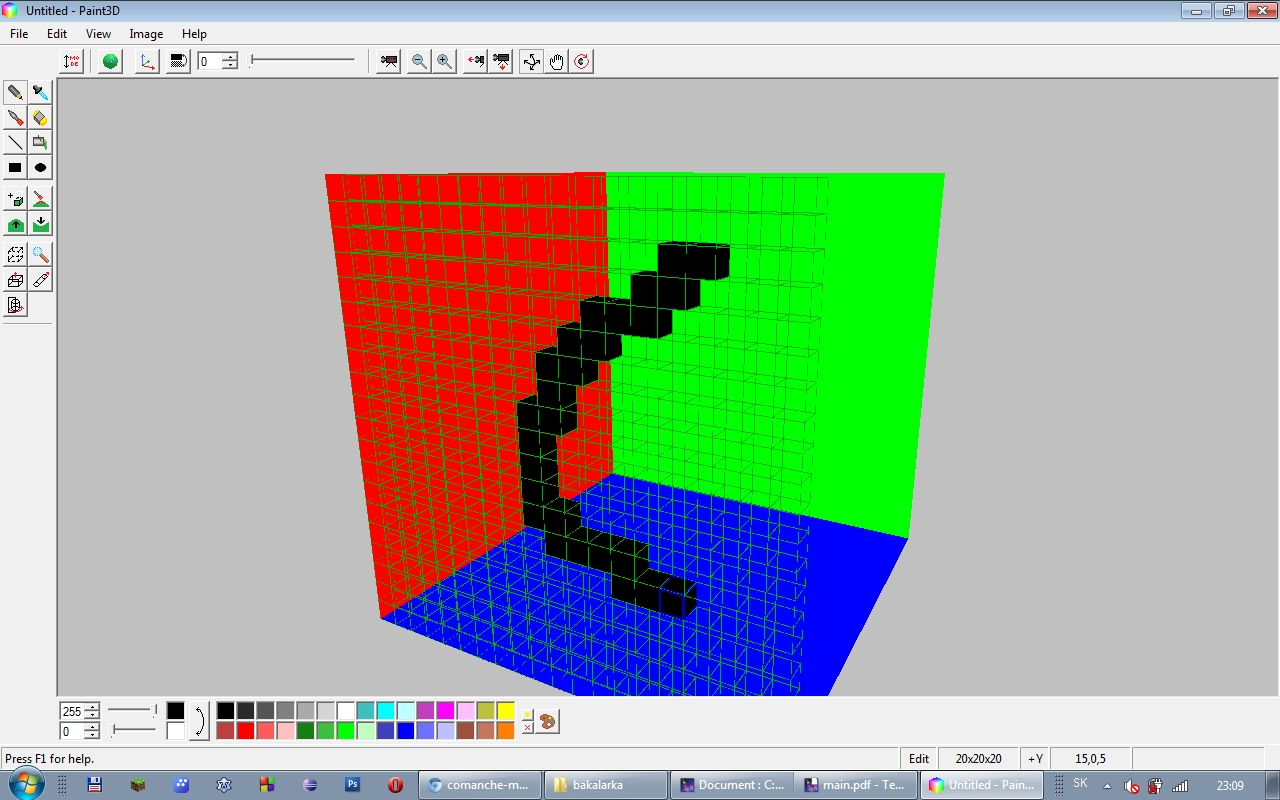
\includegraphics[width=0.8\textwidth]{paint3D.jpg}
	\caption[Paint3D]{Screenshot z programu Paint3D}
	\label{obr:paint3D}
\end{figure}


\subsection{Voxel3D}
Jedná sa o program od spoločnosti \textit{Everygraph} \cite{voxel3d}. Interface aplikácie je zobrazený na obrázku \ref{obr:voxel3D}.
\subsubsection{Výhody:}
\begin{itemize}
	\item \textbf{Voxelizácia}. Ako jediný z testovaných ponúka možnosť voxelizície 3D meshu. Taktiež umožňuje počas tvorby zobraziť tento mesh spolu s voxelizovaným objektom a podľa ľubovôle ho umiestňovať. 
	\item \textbf{Jednoduchý interface}. V programe sa dá ľahko zorientovať, a preto je vhodný aj pre neskúsených užívateľov.
	\item \textbf{4 rôzne náhľady}. Táto funkcionalita je bežná v 3D modelovacích nástrojoch, avšak toto je jediný z testovaných voxelových editorov, ktorý ju obsahuje.
	\item \textbf{Import/Export}. Výhodou programu je, že má vlastný binárny a aj ASCII formát na ukladanie dát. Taktiež program ponúka aj export do .obj formátu. Nevýhodou však je, že program nepodporuje žiadne iné bežne používané voxelové formáty.
\end{itemize}
\subsubsection{Nevýhody:}
\begin{itemize}
	\item  \textbf{Rýchlosť}. Tento parameter dosahuje nedostatočné hodnoty najmä pri vytváraní prázdneho objektu. Už pri pomerne malých rozmeroch vytvorenie objektu trvá iritujúco dlho. Pri testovaní sme vytvárali objekt s počtom voxelov \begin{math}32^3\end{math} a ďalší objekt mal počet voxelov \begin{math}64^3\end{math}. Vytvorenie prvého objektu trvalo približne 6 sekúnd, zatiaľ čo vytvorenie druhého trvalo približne 48 sekúnd.
	\item \textbf{Neošetrené vstupy}. Napriek tomu, že je program pomalý aj pri malých rozmeroch, jeho interface umožňuje vytvoriť objekt s počtom voxelov \begin{math}(2^{32})^3\end{math}.
	\item \textbf{Zdĺhavé modelovanie}. Očakávame, že tvorba voxelových objektov nebude najrýchlejšia, avšak kreslenie voxelov v tomto programe je o to zdĺhavejšie, že umožňuje kresliť iba po rezoch objektom.
	\item \textbf{Jeden objekt v scéne.} Možnosť pridávania viacerých objektov do scény neumožňuje väčšina programov.
\end{itemize}

\begin{figure}[ht!]
	\centering
	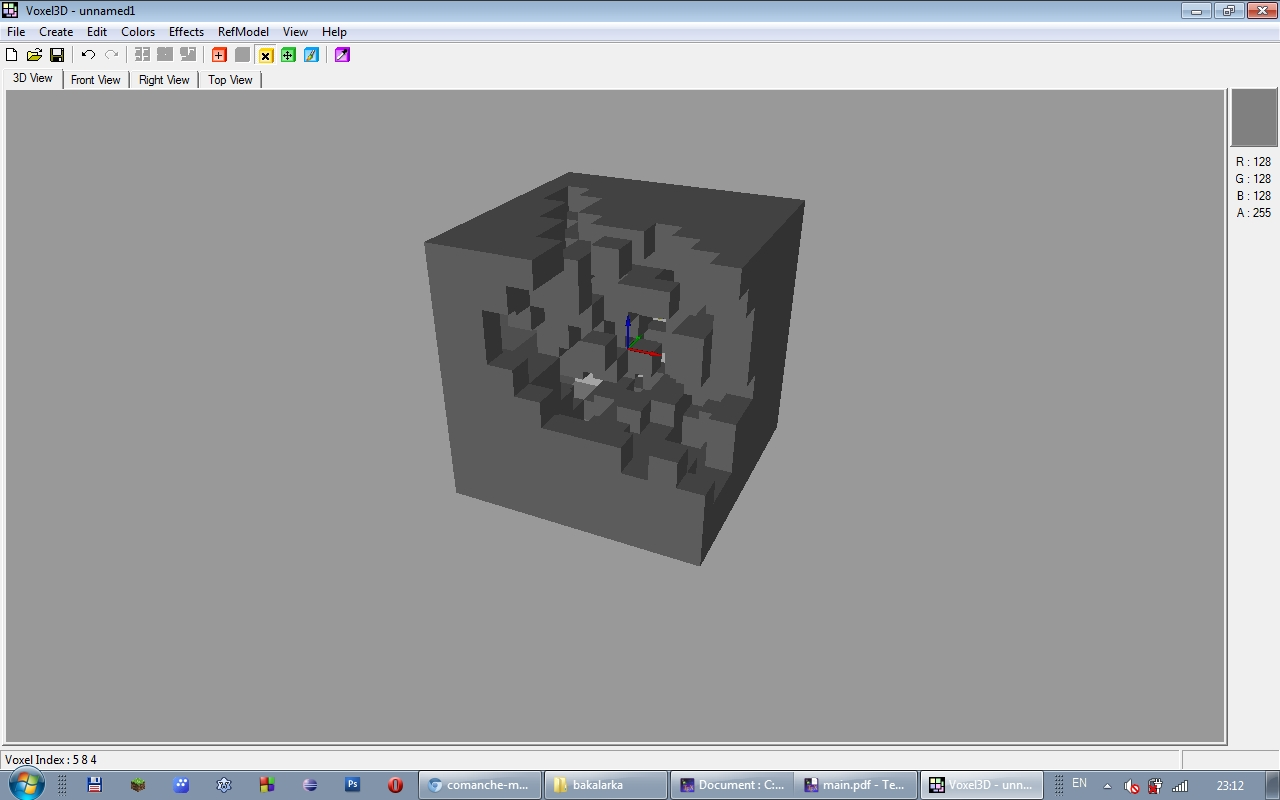
\includegraphics[width=0.8\textwidth]{Voxel3D.jpg}
	\caption[Voxel3D]{Screenshot z programu Voxel3D}
	\label{obr:voxel3D}
\end{figure}

\subsection{3D Dot Game Hero Editor}
Táto aplikácia je skôr online editor, pre tvorbu voxelových hrdinov do hry 3D Dot Game \cite{dotGame}. Interface aplikácie je zobrazený na obrázku \ref{obr:hero}.
\subsubsection{Výhody:}
\begin{itemize}
	\item \textbf{Dostupnosť cez prehliadač}. Tento fakt je aj výhodou, ale aj nevýhodou daného programu, pretože je dostupný výlučne cez prehliadač a neexistuje desktopová verzia.
	\item \textbf{Jednoduchosť použitia}. Táto vlastnosť je zaručená najmä vďaka malému množstvu nástrojov a možností softvéru.
	\item \textbf{Render a animácia}. Ak v programe zvolíme možnosť \textit{save}, automaticky sa vyrenderuje balík výstupných súborov, ktoré sa nám ponúknu na stiahnutie. Tento balík obsahuje 2 rendery s pozadím a bez pozadia, jednu animáciu objektu (ide iba o rotáciu okolo vlastnej osi) a jeden wallpaper. 
\end{itemize}

\subsubsection{Nevýhody:}
\begin{itemize}
	\item \textbf{Ponuka nástrojov}. Ako bolo spomenuté, program ponúka iba chudobné množstvo editovacích nástrojov v počte 3.
	\item \textbf{Obmedzenie farieb}. Taktiež aj farebná paleta je obmedzená na niečo viac ako tucet farebných odtieňov.
	\item \textbf{Obmedzené rozmery}. Tvorený objekt je ohraničený bounding boxom, ktorý nemožno nijak prekročiť, ani zmeniť jeho rozmery.
	\item \textbf{Export/Import}. V ponuke aplikácie nie je žiaden import a exportovať je možné iba render, ako bolo spomenuté vyššie.
	\item \textbf{Jeden objekt v scéne.} Možnosť pridávania viacerých objektov do scény neumožňuje väčšina programov.
\end{itemize}

\begin{figure}[ht!]
	\centering
	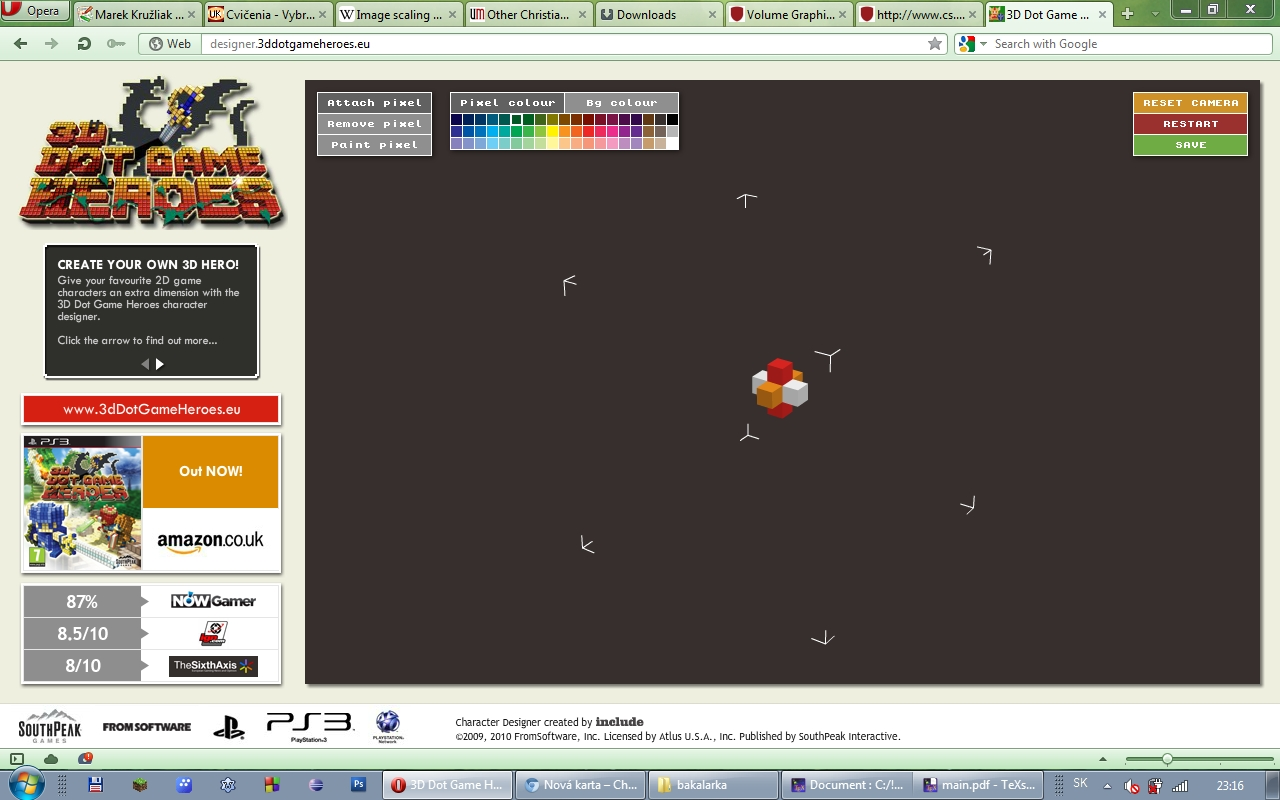
\includegraphics[width=0.8\textwidth]{3Dhero.jpg}
	\caption[3D Dot Game Hero Editor]{Screenshot z programu 3D Dot Game Hero Editor}
	\label{obr:hero}
\end{figure}


\subsection{Zoxel}
Zoxel je kvalitný výtvor od jediného človeka menom Graham King \cite{zoxel}. Interface aplikácie je zobrazený na obrázku \ref{obr:zoxel}.
\subsubsection{Výhody:}
\begin{itemize}
	\item \textbf{Lepší shading}. Väčšina programov používa pre tieňovanie jednoduchý flat-shading zatiaľ, čo Zoxel má implementovaný istý druh smooth-shadingu, resp. využíva základný z možností OpenGL knižnice.
	\item \textbf{Jednoduchý interface}. Interface je jednoduchý a intuitívny s možnosťou ľubovolného premiestňovania niektorých komponentov, ako napríklad paleta farieb alebo nástrojov.
	\item \textbf{Wireframe}. Program umožňuje zobraziť model ako wireframe.
	\item \textbf{Interaktívne rozširovanie voxelového priestoru}.
	\item \textbf{Import/Export}. Výhodou programu je, že má vlastný binárny formát na ukladanie dát. Taktiež program ponúka aj export do .obj formátu a ukladanie a náčítanie súboru z programu Sproxel spomenutého nižšie.
\end{itemize}
\subsubsection{Nevýhody:}
\begin{itemize}
	\item \textbf{Kamera}. Pri testovaní nám najväčšie problémy spôsobovala nemotorná kamera, ktorá občas prejavovala neočakávané správanie.
	\item \textbf{Kreslenie}. Kreslenie je vyriešené veľmi nešťastne, kedže sa dá pridať iba jeden voxel na klik. Teda nie je umožnené kreslenie na udalosť ťahania myši.
	\item \textbf{Chudobná ponuka nástrojov}.
	\item \textbf{Jeden objekt v scéne.} Možnosť pridávania viacerých objektov do scény neumožňuje väčšina programov.
\end{itemize}

\begin{figure}[ht!]
	\centering
	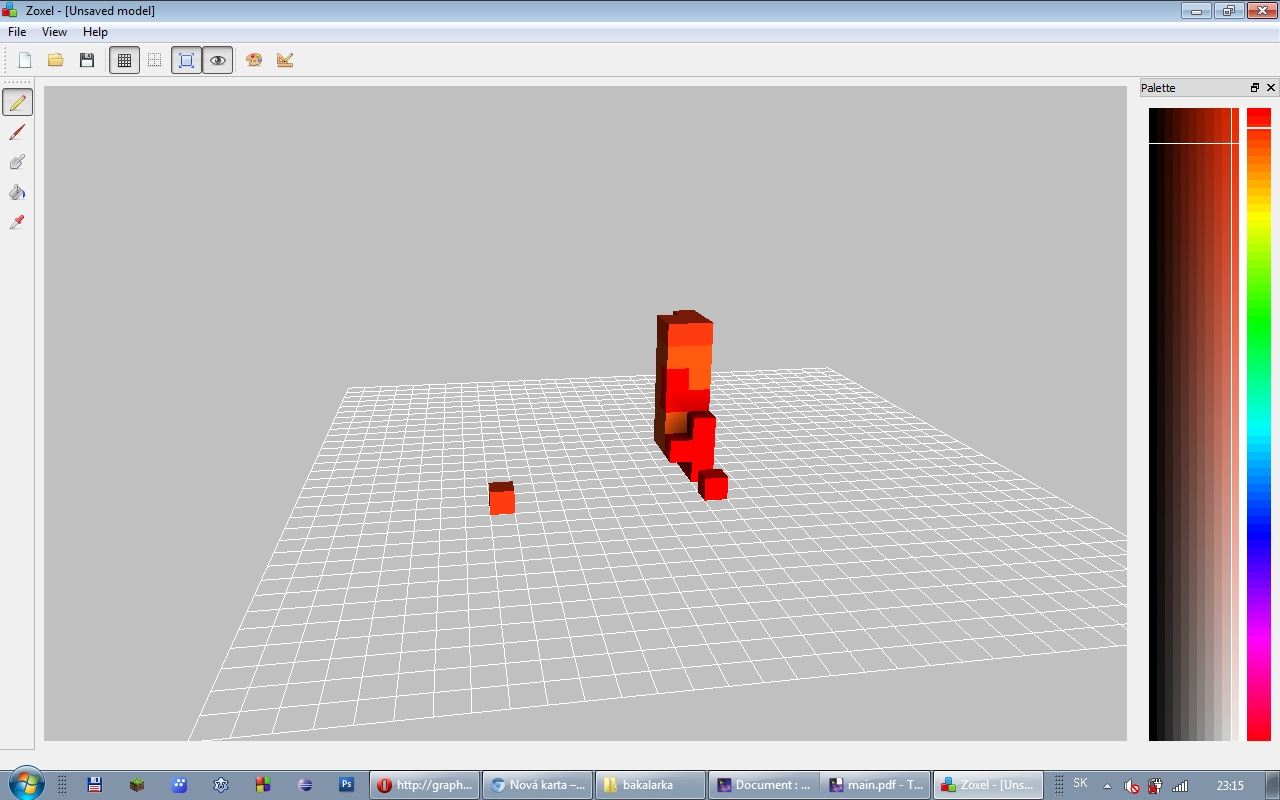
\includegraphics[width=0.8\textwidth]{zoxel.jpg}
	\caption[Zoxel]{Screenshot z programu Zoxel}
	\label{obr:zoxel}
\end{figure}

\subsection{Sproxel}
Horlivo vyvíjaný voxelový editor, tak by sa dal charakterizovať Sproxel \cite{sproxel}. Interface aplikácie je zobrazený na obrázku \ref{obr:sproxel}.
\subsubsection{Výhody:}
\begin{itemize}
	\item \textbf{Jednoduché ovládanie}. Program mal jedno z najlepších ovládaní a nebolo vôbec zložité sa ho naučiť.
	\item \textbf{Jednoduchý interface}. Interface je jednoduchý a intuitívny s možnosťou ľubovoľného premiestňovania niektorých komponentov, ako napríklad paleta farieb alebo nástrojov.
	\item \textbf{Ponuka nástrojov}. Ponuka nástrojov a rôznych úprav je dostačujúca a v porovnaní s niektorými programami až nadpriemerná.
	\item \textbf{Export/import}. Okrem vlastného binárneho súborového formátu na ukladanie a načítavanie objektov má aplikácia v ponuke aj rôzne druhy importu a exportu napríklad ako .obj alebo ako obrázok vo formáte .png a mnohé iné.
	\item \textbf{Medziplatformovosť}. 
	\item \textbf{Aktívny vývoj}. Aj v súčasnosti sa aktívne pracuje na vývoji tohto softvéru. Najnovšia verzia je Sproxel 0.6, takže nám vývojári pravdepodobne sľubujú ešte niekoľko ďalších verzií.
\end{itemize}
\subsubsection{Nevýhody:}
\begin{itemize}
	\item \textbf{Z-fighting}. Problém z-fightingu nie je riešený ani na miestach, kde by to bolo pomerne jednoduché. Jeho neriešenie spôsobuje nie len neestetickosť výsledku ale aj neprehľadnosť pri práci s voxelmi.
	\item \textbf{Voxel grid}. Čo by mohlo byť výhodou, je však nevýhodou, pretože zapnutie zobrazenia voxel gridu spôsobuje v podstate zaseknutie programu už pri počte voxelov \begin{math}32^3\end{math}.
	\item \textbf{Jeden objekt v scéne.} Možnosť pridávania viacerých objektov do scény neumožňuje väčšina programov.
\end{itemize}

\begin{figure}[ht!]
	\centering
	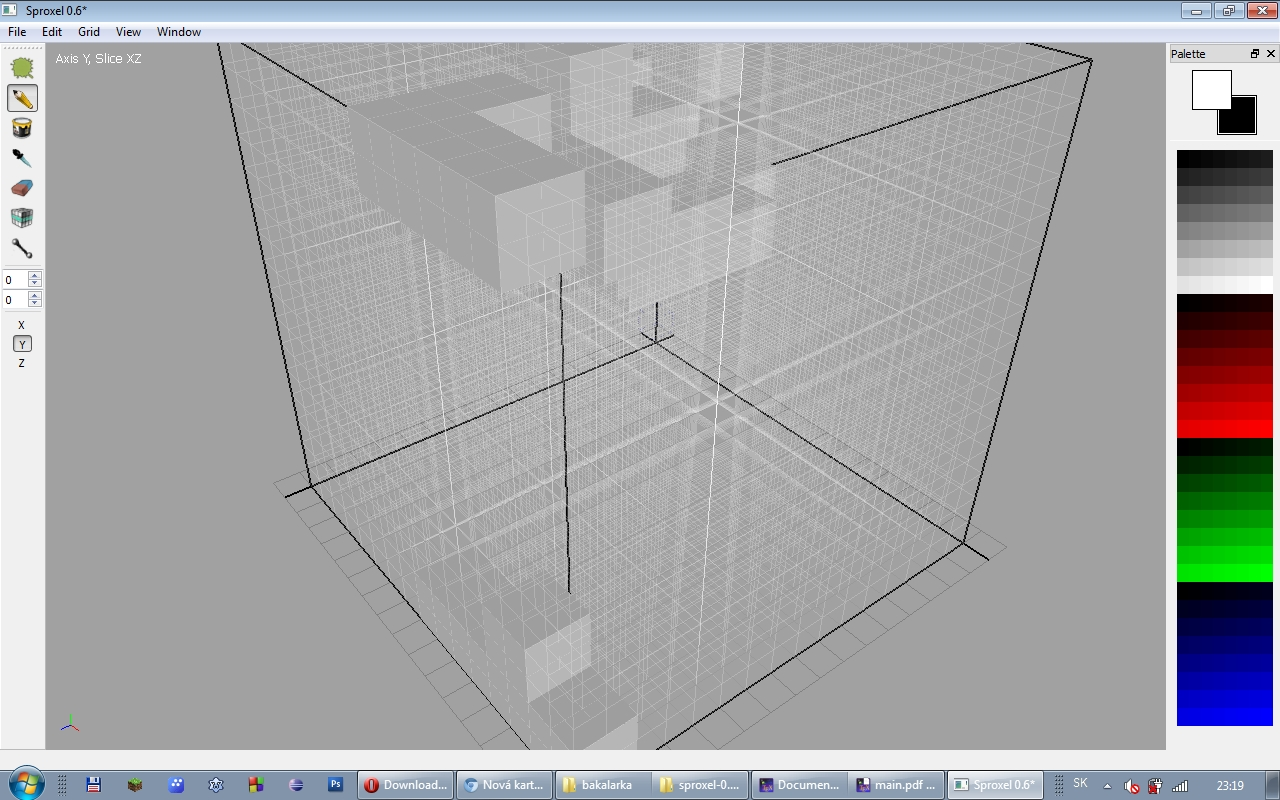
\includegraphics[width=0.8\textwidth]{sproxel.jpg}
	\caption[Sproxel]{Screenshot z programu Sproxel}
	\label{obr:sproxel}
\end{figure}

\eject

\subsection{Qubicle}
Qubicle je veľmi kvalitný softvér od spoločnosti minddesk \cite{qubicle}. Interface aplikácie je zobrazený na obrázku \ref{obr:qubicle}.
\subsubsection{Výhody:}
\begin{itemize}
	\item \textbf{Ponuka nástrojov a funkcií}. Aplikácia sama o sebe neponúka veľké množstvo nástrojov, avšak ich počet je dostačujúci a sú doplnené ohromným množstvom funkcií a nastavení na úpravu objektov a scén.
	\item \textbf{Interface.} Prostredie je pomerne jednoduché s obzvlášť peknou grafikou.
	\item \textbf{Viacej objektov v scéne}. Tento program ako jediný z testovaných ponúka možnosť vytvárania viacerých nezávislých objektov v scéne, čo umožňuje lepšiu variabilnosť pri tvorbe.
	\item \textbf{Defaultné tvary}. Okrem prázdneho objektu je možné pridať základné objemové útvary ako napríklad kváder, ihlan, elipsoid, valec a kužel. Taktiež je možné vygenerovať náhodný voxelový terén. Táto možnosť je však až v platenej verzii, preto sme ju nemohli otestovať.
	\item \textbf{Editačné módy}. Rozličné módy editovania nám umožňujú tvoriť na troch rozličných leveloch. Na úrovni scény, na úrovni objektu a na úrovni rezu. Vďaka tomu máme pomerne veľkú kontrolu nad tým, čo robíme. 
	\item \textbf{Import/Export}. Program má vlastný binárny formát na ukladanie a na načítavanie súborov. Taktiež je možný export do XML, .obj alebo do rôznych známych binárnych voxelových formátov.
	\item \textbf{Lokalizácia}. V nastaveniach programu je možné vybrať jeden zo štyroch svetových jazykov.
	\item \textbf{Rendering}. Ako jeden z mála programov, má \textit{Quibicle} zabudovaný jednoduchý rendering objektov s obrázkovým súborom ako výstupom.
\end{itemize}
\subsubsection{Nevýhody:}
\begin{itemize}
	\item \textbf{Licencia}. Voľne stiahnuteľná je iba \textit{Basic} verzia programu, ktorá sa dá použiť výlučne na nekomerčné účely. Táto verzia nezahŕňa širšiu funkcionalitu a export objektov. Vyššie verzie sú platené.
	\item \textbf{Komplikovanosť}. Veľké množstvo funkcií a nastavení vyžaduje viacej času naučiť sa dokonale ovládať tento nástroj. Avšak základy je veľmi ľahké pochytiť a sú dostačujúce na dosiahnutie pomerne dobrých výsledkov.
\end{itemize}

\begin{figure}[ht!]
	\centering
	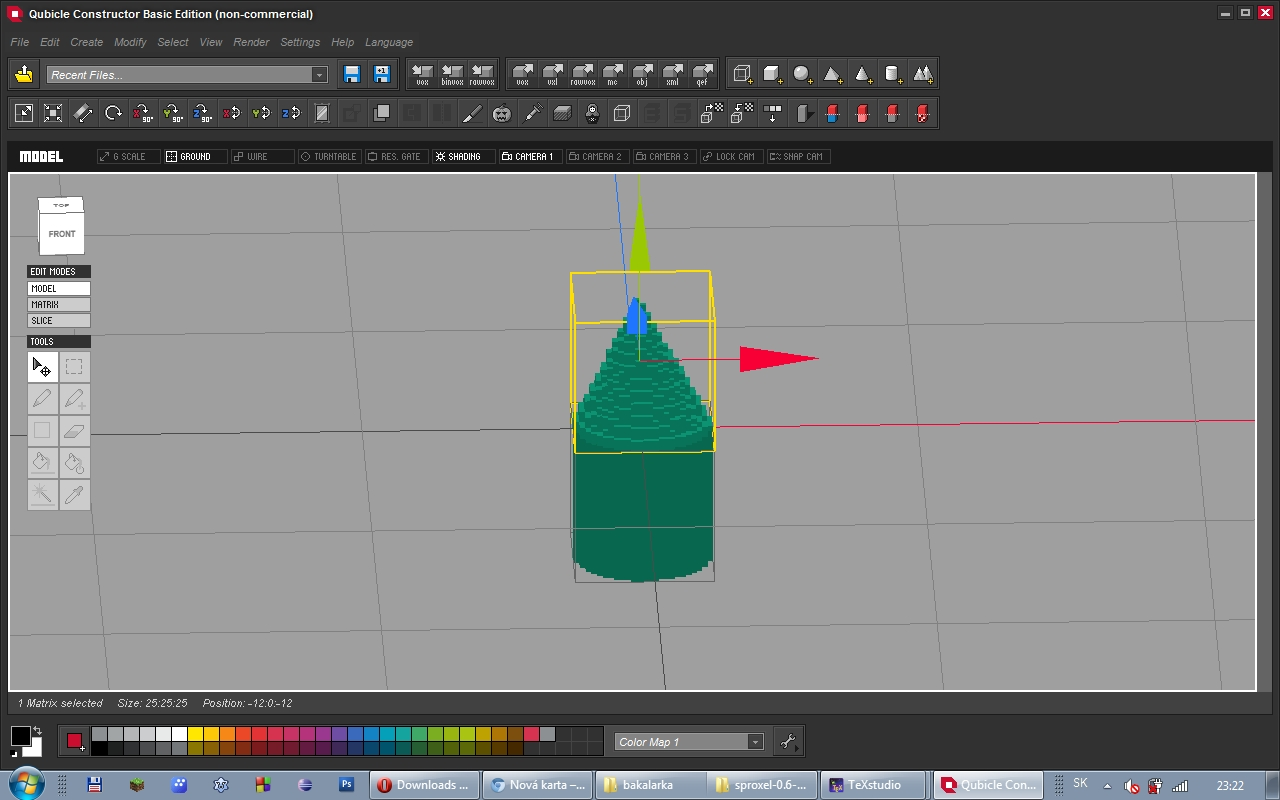
\includegraphics[width=0.8\textwidth]{qubicle2.jpg}
	\caption[Qubicle]{Screenshot z programu Qubicle}
	\label{obr:qubicle}
\end{figure}

\section{2D grafické editory}
Keďže si predstavujeme prácu s voxelmi ako kreslenie objektov v priestore, inšpiráciou nám pre našu prácu bolo mnoho 2D kresliacich programov akými sú napríklad \textit{Adobe Photoshop}, \textit{Gimp} alebo jednoduchší \textit{Microsoft Paint}. Tieto aplikácie poskytujú užívateľovi širokú sadu nástrojov, z ktorých sme sa rozhodli niektoré z nich použiť aj my. Taktiež sme sa snažili pri vytváraní GUI a nastavovaní spôsobu používania nástrojov vytvoriť podobný pocit, ako pri práci napríklad v programe MsPaint.

\section{Zhrnutie poznatkov z testovania}
Prieskum spomínaného softvéru nám umožnil vytvoriť si detajlnejší obraz o našich cieľoch a možnostiach pri implementácii práce. 
Najlepšie výsledky v testovaní dosiahol jednoznačne program Qubicle. Jeho filozofiou modelovania sme sa najväčšmi stotožnili, kedže ako jediný umožňoval vytvárať samostatné objekty, ktoré bolo následne možné ľubovoľne umiestniť v scéne. Taktiež obsahoval najväčšie množstvo funkcií a aj napriek tomu mal rýchlo pochopiteľný interface. Jeho najslabšou stránkou teda zostáva, že jeho plná verzia je platená.
Zvyšné programy nedosahovali podobné výsledky, avšak vytvorili spodnú hranicu kvality, ktorú by chcela dosiahnuť aj táto práca.



\chapter{Implementácia}\label{chap:implementacia}
Začiatkom tejto kapitoly v stručnosti opisujeme použité technológie a taktiež uvádzame dôvody, prečo sme si ich zvolili. 
Jednotlivé časti programu sme zhrnuli do viacerých súvislých celkov, ktoré sme podrobne charakterizovali a preskúmali. Najdôkladnejšie sa venujeme častiam programu, ktoré považujeme za zaujímavé, z dôvodov ich zložitosti alebo kvôli metóde, ktorú sme pri ich riešení použili. 

\section{Použité technológie}

\subsection{C++}
Jazyk C++ vznikol rozšírením jazyka C o triedy a iné rysy objektovo orientovaného programovania. Jedná sa o 
jeden z najznámejších a najobľúbenejších programovacích jazykov za posledných pár dekád. Vďaka jeho obľúbenosti bolo vytvorených mnoho interných ale aj externých knižníc a nadstávb, čo je jeden z dôvodov, prečo sme si ho zvolili na prácu. 

Vďaka tomu, že má tento jazyk nízkoúrovňové a zároveň aj vysokoúrovňové črty programovacích jazykov, umožňuje dobrý interface na efektívny manažment pamäťových a procesových zdrojov. Spomínaná vlastnosť jazyka je užitočná pri pamäťovo a výpočtovo náročných algoritmoch, s ktorými sa pri objemovej grafike zaručene stretneme.

\subsection{OpenGL}
V práci sme si ako prvé uvedomili nevyhnutnosť vizualizácie voxelového priestoru a na túto úlohu sme vybrali knižnicu OpenGL.

Jedná sa o jednu z najznámejších a najpoužívanejších open source multi-platformových API na interakciu s grafickými akcelerátormi (GPU). Dobre špecifikovaný OpenGL štandard má jazykové väzby na mnohé často používané programovacie jazyky \cite{OpenGL}.
Funkcie OpenGL API sú dobre definované a sú volateľné aj z jazyka C++, ktorý sme si zvolili ako hlavnú implementačnú technológiu. Táto knižnica vo všeobecnosti ponúka široké množstvo výhod, akou je napríklad veľké množstvo podrobných rád a návodov, ako s knižnicou narábať a zároveň má OpenGL veľmi podrobne spracovanú dokumentáciu. Aj toto bol jeden z dôvodov, prečo sme si ju zvolili pre náš účel.

%Aby sme vedeli efektívne využívať možnosti, ktoré nám OpenGL ponúka, je potrebné nahliadnuť trocha pod povrch tejto knižnice na renderovaciu pipeline.
%
%Ako možno vidieť na obrázku \ref{pipeline} ... strucny opis pipeline
%
%
%\begin{figure}[ht!]
%	\centering
%	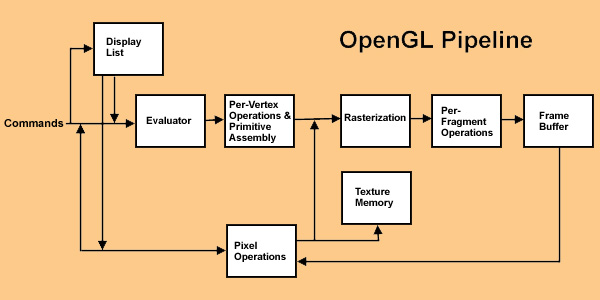
\includegraphics[width=90mm]{pipeline.JPG}
%	\caption{OpenGL pipeline}
%	\label{pipeline}
%\end{figure}

\subsection{DevIL}
Počas implementácie sa ukázalo, že je potrebné načítať bitmapy, ktoré sa následne použili ako textúry, alebo sa pretransformovali na jednovrstvový voxelový objekt. Ako prvá sa nám ponúkla knižnica \textit{DevIL} \cite{devil}, ktorú sme nakoniec aj v práci použili.

DevIL, pôvodne pomenovaná ako OpenIL, je programátorská knižnica, slúžiaca na načítavanie obrázkov širokej škály formátov do pamäti. Udržiava podobné menné konvencie ako OpenGL a veľmi dobre s ním aj spolupracuje.

\subsection{Microsoft Visual Studio 2012}
Spoločnosť \textit{Microsoft} ponúka vysokokvalitné vývojové prostredie \textit{Microsoft Visual Studio} \cite{mvs}, ktoré je pre študentov našej fakulty dostupné zdarma a voľne použiteľné na nekomerčné účely.
Jeho integrovanou súčasťou je aj prostredie na vytváranie GUI pre Win32, čo je jeho hlavná výhoda, ktorú sme zohladňovali pri výbere toho správneho IDE.
V prvých fázach práce sme volili verziu 2010 Express, ktorá však neobsahovala možnosť lepšieho syntax highlightu, čo bolo pri rozsiahlosti kódu pomerne dôležité, a tak sme nakoniec prešli na verziu 2012, ktorá nám plne vyhovovala.

\subsection{Assimp}
Na loadovanie povrchových modelov za účelom voxelizácie sme vybrali knižnicu \textit{Assimp} \cite{assimp}, ktorá je taktiež voľne dostupná.

Jej hlavnými výhodami sú, že poskytuje pre a post-processing, má jednoduchý interface a podporuje tucty rôznych 3D súborových formátov.

Nevýhodami naopak sú, že má komplikovanejšiu inštaláciu, niektoré zdokumentované triedy nie sú správne implementované alebo nie su implementované vôbec a to často spôsobuje problémy, ktoré sa môžu objaviť pri práci.
\subsection{pugixml}
Na export a import dát z celej scény sme sa rozhodli použiť jazyk XML a nami navrhnutú podrobnú štruktúru opisujeme nižšie v tejto kapitole. Keďže parsovanie takýchto štruktúr nie je úplne triviálne a je vytvorených už mnoho existujúcich riešení, využili sme túto možnosť a siahli po knižnici \textit{pugixml} \cite{pugixml} na parsovanie XML súborov.

Dôvodom prečo sme si ju zvolili je, že sa jedná o extrémne rýchlu knižnicu, ktorá vytvorí DOM strom z XML súboru, takže zaručuje jednoduché použitie.

\section{Rendering}
Na rendering sme použili spomínanú knžinicu OpenGL s jej programovým rozšírením OpenGL Utility Toolkit (GLUT) \cite{glut}.
\subsection{Rendering voxelu}
Predpokladáme, že voxel ako základný element voxelového priestoru sa bude v scéne nachádzať v pomerne veľkých objemoch. Z tohoto dôvodu bolo potrebné nájsť spôsob, ako jeden voxel čo najúspornejšie vyrenderovať.
Na tento účel sme sa rozhodli použiť display listy. Display list je séria príkazov OpenGL, ktoré sú skompilované a uložené, spolu s inými dátami o objekte na GPU \cite{DisplayList}.
Vďaka tomu používanie displaylistov redukuje komunikáciu medzi GPU a CPU, ktorá je v procese renderovania časovo náročná. Display listy sú teda vhodné na rendering objektov s rovnakou topológiou, ktoré sa v scéne vyskytujú veľmi často. Keďže každý voxel je objekt v tvare kocky s rôznymi vlasnosťami akou je napríklad farba, môžme použiť jedinú zabudovanú funkciu GLUTu: 
\begin{verbatim}
   void glutSolidCube(GLdouble size)
\end{verbatim}
alebo tiež:
\begin{verbatim}
   void glutWireCube(GLdouble size)
\end{verbatim}
Spôsob renderovania voxelu ešte ovplyvňujú jeho vnútorné vlastnosi ako farba, flag určujúci označenie voxelu, a taktiež nastavenie renderingu ako napríklad shading, backface culling, zobrazenie wireframu alebo tiež veľkosť vzorky.
\subsection{Rendering objektu}
Ako sme spomenuli o sekciu vyššie, bolo potrebné nájsť spôsob ako čo najviac ušetriť renderovací proces. Takéto vylepšenie je možné spraviť aj pri renderingu objektov, pretože veľké množstvo voxelov býva prekrytých inými. Použili sme preto veľmi jednoduchú, ale účinnú metódu, ktorá rozhoduje, či voxel zobraziť, podľa toho, io je ohraničený zo všetkých šiestich strán alebo nie je. Takto sme sa zbavili vykreslovania všetkých voxelov, ktoré nebolo možné nikdy vidieť.
\subsection{Rendering scény}
Scéna sa skladá z viacerých voxelových objektov, ktoré je potrebné pri zobrazovaní posunúť správnou translačnou maticou na svoju pozíciu. Plávajúce objekty v priestore môžu na užívateľa programu pôsobiť dezorientujúco, a preto sme pridali do scény dva vizuálne elementy a tými sú podlaha a začiatok karteziánskej sústavy s troma osami. 


\section{Voxelové Objekty}\label{voxelObjects}
Sekundárny element v našom priestore po voxeloch je voxelový objekt, ktorý o sebe uchováva sadu základných informácií, z ktorých najdôležitejšie sú pozícia, dané rozmery a voxely, ktoré mu prislúchajú.

Každý objekt v scéne predstavuje samostatný ohraničený voxelový priestor. Na jeho reprezentáciu sme sa rozhodli použiť trojrozmerné pole, ktorého výhodou je priamy prístup k voxelom prostredníctvom ich indexov.
Vďaka tejto vlastnosti je možné rýchlo a jednoducho procedurálne generovať voxelové objekty a ich rôzne transformácie.

\subsection{Základné tvary}
Pre jednoduchšie a rýchlejšie modelovanie väčšina 3D grafických nástrojov ponúka sadu základných telies, ktoré sú pri práci často využívané. Takýmto postupom sme sa inšporovali i my a zhotovili sme sadu objektov\footnote{Kôli diskrétnosti voxelového priestoru, spomenuté objekty predstavujú iba aproximáciu konkrétnych geometrických útvarov.}, ktoré sa generujú na základe jednoduchej matematiky. Takéto generovanie by sme mohli zovšeobecniť na nasledujúci algoritmus:


\begin{algorithmic}
	\For{$(i,j,k) = (0,0,0) \to (width, height, depth)$}
		\If{ $v\_telese(i,j,k)$ } // funkcia je špecifická pre každý útvar
			\State Pridaj voxel do $Objekt$u na pozíciu (i,j,k)
		\Else
			\State Pridaj $NULL$ do $Objekt$u na pozíciu (i,j,k)
		\EndIf
	\EndFor
\end{algorithmic} 

	\subsubsection{Kváder}
	Vytvorenie kvádra je veľmi jednoduché. Jeho podmienka v spomenutom algoritme je funkcia vracajúca vždy hodnotu \textit{TRUE}. Takúto funkciu môžme odstrániť a v jednoduchosti môžme povedať, že objekt inicializovaný na dané rozmery iba naplníme voxelmi príslušnej farby.
	\subsubsection{Elipsoid}
	Elipsoid je povrchové teleso dané rovnicou:
	\begin{displaymath}
	\frac{x^2}{a^2} + \frac{y^2}{b^2}+ \frac{z^2}{c^2} = 1 
	\end{displaymath}
	Keďže v našom prípade budeme potrebovať elipsoid so stredom v bode \\ \begin{math}S = (s_1,s_2,s_3)\end{math}
	k úžitku nám bude všeobecnejšia rovnica:
	\begin{displaymath}
		\frac{(x - s_1)^2}{a^2} + \frac{(y - s_2)^2}{b^2}+ \frac{(z - s_3)^2}{c^2} = 1 
	\end{displaymath}
	Kde \textit{a}, \textit{b}, \textit{c} určujú dĺžky poloosí v smere osí \textit{x}, \textit{y}, \textit{z} ako možno vidieť na obrázku \ref{elipsoid}.
	
	Vďaka tejto rovnici môžme ľahko určiť, ktoré body sa nachádzajú v telese alebo mimo telesa, vytvorením nerovnice, ktorá vznikne nahradením znamienka = za \begin{math} < \end{math} alebo \begin{math} > \end{math}.

	\begin{figure}[ht!]
	\centering
	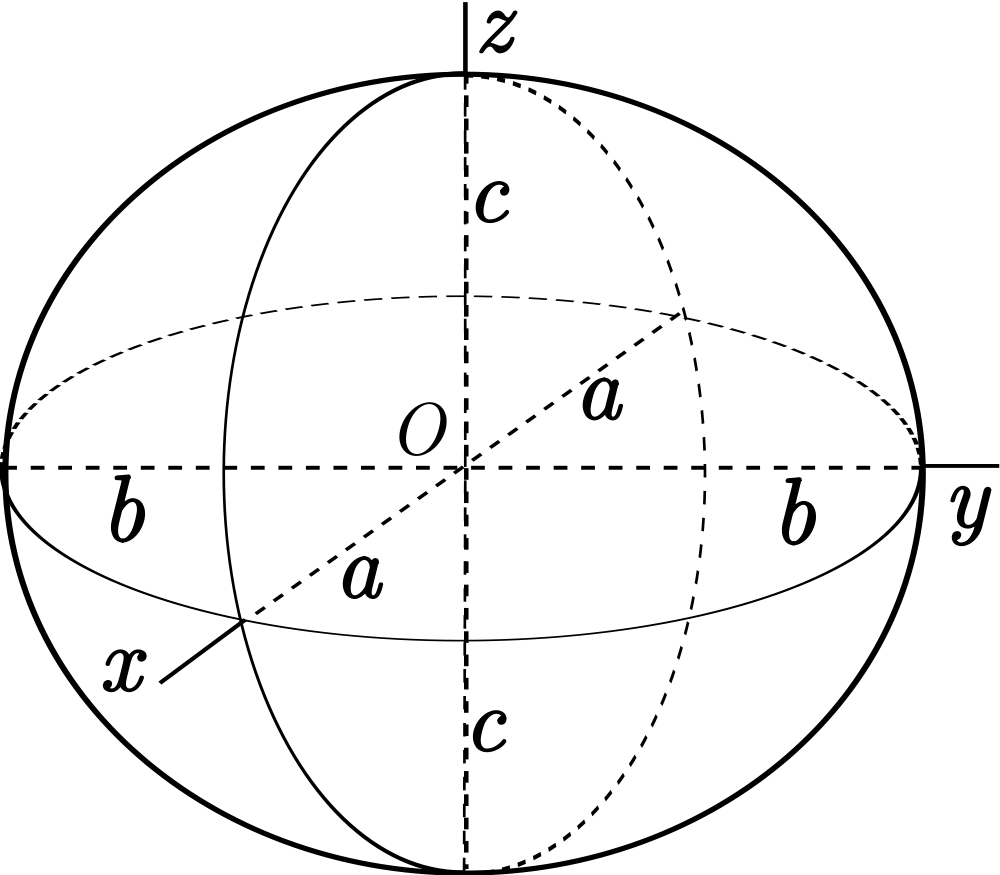
\includegraphics[width=90mm]{ellipsoid.png}
	\caption{Elipsoid}
	\label{elipsoid}
	\end{figure}
	
	V našom prípade sú hodnoty \textit{a}, \textit{b}, \textit{c} nahradené za \textit{width/2}, \textit{height/2}, \textit{depth/2}, hodnoty \textit{x}, \textit{y}, \textit{z} za \textit{i}, \textit{j}, \textit{k} a stred S = (width/2, height/2, depth/2). Naša funkcia rozhodujúca, či sa voxel nachádza v telese by mohla vyzerať takto:
	\begin{displaymath}
		\frac{(i - (width/2))^2}{(width/2)^2} + \frac{(j-(height/2))^2}{(height/2)^2}+ \frac{(k - (depth/2)) ^2}{(depth/2)^2} < 1 
	\end{displaymath}
	zjednodušene:
	\begin{displaymath}
			\frac{(i - s_1)^2}{s_1^2} + \frac{(j-s_2)^2}{s_2^2}+ \frac{(k - s_3) ^2}{s_3^2} < 1 
	\end{displaymath}
	a ešte jednoduchšie:
	\begin{displaymath}
		(\bar{p})^2 < 1 \textrm{, kde }
		\bar{p} = (\frac{i - s_1}{s_1}, \frac{j - s_2}{s_2}, \frac{k - s_3}{s_3}) 
	\end{displaymath}
	\subsubsection{Valec}
	Základ na vygenerovanie valca je podobný ako pre elipsoid, s tým rozdielom, že potrebujeme rovnicu posunutej elipsy do stredu \begin{math}S = (s_1, s_2)\end{math} :
	\begin{displaymath}
		\frac{(x - s_1)^2}{a^2} + \frac{(y - s_2)^2}{b^2} = 1 
	\end{displaymath}
	Pre každú vrstvu objektu v našom prípade v smere osi \textit{y} (zanedbávame teda y-ovú súradnicu respektíve súradnicu j) zisťujeme, či sa bod nachádza v elipse alebo mimo nej. Táto elipsa je určená stredom \begin{math}S = (wdith/2, depth/2)\end{math} a rovnakými rozmermi, teda \begin{math}a = wdith/2, b = height/2\end{math}. Výsledná nerovnica vyzerá nasledovne:
	\begin{displaymath}
		\frac{(i - (width/2))^2}{(width/2)^2} + \frac{(k - (depth/2)) ^2}{(depth/2)^2} < 1  
	\end{displaymath}
	Toto môžme zjednodušiť rovnako ako v predchádzajúcom prípade na:
	\begin{displaymath}
		(\bar{p})^2 < 1 \textrm{, kde }
		\bar{p} = (\frac{i - s_1}{s_1},\frac{k - s_3}{s_3})
	\end{displaymath}	
	\subsubsection{Ihlan}
	Pre pochopenie základného konceptu tvorby diskrétneho ihlanu, môžme problém zjednodušiť na vygenerovanie diskrétneho rovnoramenného trojuholníka.
	Počet bodov pre prvý a posledný riadok takéhoto trojuholníka vieme ľahko zistiť. Prvý riadok obsahuje 1 alebo 2 body podľa toho, či je šírka trojuholníka párna alebo nepárna, no a posledný riadok obsahuje počet bodov rovný šírke trojuholníka. Aby sme získali počet bodov, ktoré sa nachádzajú v riadkoch medzi prvým a posledným, stačí nám použiť lineárnu interpoláciu bodov: 
	$X = (x,y), A = (x_0, y_0), B = (x_1, y_1)$ 
	\begin{displaymath}
	\frac{y - y_0}{x - x_0} = \frac{y_1 - y_0}{x_1 - x_0} 
	\end{displaymath}
	Pre nás je x hľadaný počet bodov na riadok $j$, y je spomenutý riadok $j$, $A = (f , 1)$, kde $f$ je 1 alebo 2 a $B = (width, height)$. Z toho nám vyplýva:
	\begin{displaymath}
		x = \frac{(j - 1) . (width - f)}{height - 1} + f
	\end{displaymath}
	Teraz nám už stačí umiestniť body na stred dvojrozmernej mapy, čo je pomerne jednoduché.
	Túto myšlienku pre diskrétny trojuholník už ľahko rozšírime do priestoru.
	\subsubsection{Kužeľ}
	Kužeľ je najkomplikovanejším tvarom, z pomedzi všetkých spomínaných. Avšak nie je potrebné vymýšlať nijaký nový spôsob na jeho vytvorenie, keďže tento tvar získame kombináciou už dvoch vyššie spomenutých metód. Vďaka metódam pre valec a pre ihlan môžme získať veľmi pekný voxelový kužeľ.


\subsection{Booleanovské operácie nad objektami}
Známa modelovacia paradigma CSG využíva na vytvorenie výsledného modelu booleanovské operácie. Potrebnosť tohoto prvku vo voxelovom editore sme si uvedomili aj my, a tak sme sa rozhodli implementovať základné operácie akými sú \textit{AND}, \textit{OR}, \textit{NOT} a \textit{XOR}.
Vo všobecnosti by sa dal algoritmus, ktorý sme vytvorili, pre vstupné objekty \textit{A} ,\textit{B} a výstupný \textit{C} opísať v troch krokoch:
\begin{enumerate}
\item Získanie bounding boxu pre C.
\item Zistenie pozície nového objektu C.
\item Postupné vkladanie voxelov do objektu C z objektov A,B na základe danej logickej funkcie.
\end{enumerate} 

\subsection{Transformácie objektov}
\subsubsection{Translácia}
Jedná sa o základnú transformačnú funkciu objektov, ktorej úlohou je zmeniť polohu objektu v scéne. Vyznačuje sa jednoduchou implementáciou, keďže nie je potrebné nijakým spôsobom meniť štruktúru voxelov v objekte.
V časti \ref{tools} \textit{Nástroje} v podsekcii \ref{moveTool} \textit{Posun objektov} je bližšie špecifikované ako môže užívateľ danú funkcionalitu používať.

\subsubsection{Škálovanie}
Problém vzniku dier pri škálovaní sa z 2D rasterového priestoru prenáša aj do 3D voxelového priestoru. Na jeho riešenie sme použili algoritmus \textit{Nearest-neighbor interpolation}, ktorý je veľmi jednoduchý, no napriek tomu dosahuje primerané výsledky.

Škálovať voxelový objekt je možné vo všetkých troch rozmeroch súčasne zadaním škálovacieho faktoru pre každý smer osi zvlášť.
\subsubsection{Rotácia}
Pri rotácii podobne ako pri škálovaní hrozí pri určitých hodnotách vznik dier. Tento problém sme riešili prepracovaním algoritmu na rotáciu bitmapy opísanom v článku od Michela Leunena \cite{Rotate}. 

Základnou myšlienkou je zistenie nových rozmerov obrázka a v našom prípade objektu pomocou danej rotačnej matice v priestore. Následne už len prechádzame všetkými bodmi nového objektu a snažíme sa získať voxely, pomocou spomenutej matice, z pôvodného nezrotovaného objektu. Takýmto spôsobom sme dosiahli pomerne uspokojivé výsledky.

\subsubsection{Mapovanie textúr}
Kôli jednoduchosti sme zvolili planárne mapovanie textúr na objekt podľa osí. Teda je možné namapovať textúru z celkovo 6 rôznych strán (2 pre každú os). Algoritmus mapovania textúry spočíva v štyroch krokoch:
\begin{enumerate}
\item Naškálovanie obrázka na potrebnú veľkosť. Toto zabezpečí knižnica DevIL.
\item Napasovanie obrázka na danú stenu objektu.
\item Vyslanie lúča z každého bodu obrázka smerom na objekt. \\ 
\begin{small}(Takto získame potrebný voxel.)\end{small}
\item Každý získaný voxel zafarbíme príslušnou farbou pixelu.
\end{enumerate}

\section{Nástroje}\label{tools}
Akýkoľvek editor, ktorý si predstavíte, nemôže existovať bez editačných nástrojov. V tejto časti opíšeme, aké nástroje náš voxelový editor ponúka, ich stručný opis a v prípade zaujímavých nástrojov podrobnejší opis ich implementácie.

Správu nástrojov sme riešili podľa nasledujúceho UML diagramu \ref{uml}.

\begin{figure}[ht!]
	\centering
	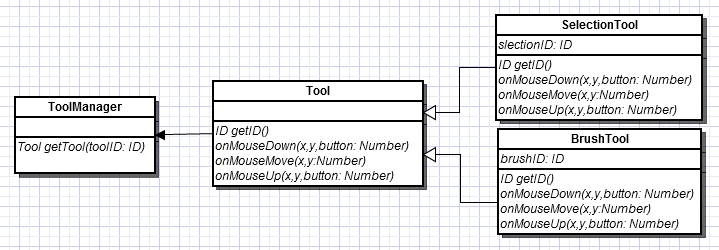
\includegraphics[width=0.9\textwidth]{tool.jpg}
	\caption{Triedny diagram pre nástroje}
	\label{uml}
\end{figure}


Základom je abstraktná trieda Tool, ktorá obsahuje virtuálne metódy:
\begin{verbatim}
   void mouseDown(int x, int y, int button)
   void mouseMove(int x, int y)
   void mouseUp(int x, int y, int button)
   ID getID()
\end{verbatim}
Hlavnou spravujúcou triedou je ToolManager, ktorý uchováva všetky objekty odvodené od triedy Tool. Vďaka spôsobu akým je manažment nástrojov navrhnutý, môžeme rôzne typy nástrojov získavať jednoducho z ToolManagera iba vďaka konkrétnemu ID.

\subsection{Selekcia}
Tento nástroj má dve funkcionality. Prvou je selekcia objektov a druhou selekcia voxelov na udalosť kliknutia na daný objekt.
\subsubsection{Selekcia objektov}
Označovanie objektov prebieha tak, že sa z miesta obrazovky vyšle lúč a následne sa zistia priesečníky so všetkými objektami v scéne. Takto získame pole objektov, z ktorých vyberieme objekt najbližší ku začiatočnému bodu lúča. Keďže predpokladáme, že voxelových objektov nebude v scéne príliš veľa, táto metóda je pre nás dostačujúca.
\subsubsection{Selekcia voxelov}
Od selekcie voxelov na kliknutie očakávame okamžitú spätnú väzbu. Ak by sme použili rovnakú metódu, ako na objekty, museli by sme zisťovať priesečníky s obrovským množstvom elementov, čo by spôsobovalo značné oneskorenie. Preto sme sa rozhodli využiť fakt, že každý voxelový objekt je umiestnený v pravidelnej trojrozmernej mriežke.

V prvej fáze zisťujeme miesto vniknutia lúču do objektu.
Na tomto mieste získame pozíciu bunky, kde by sa mohol nachádzať voxel.
Ak sa na danej pozícii žiaden voxel nenachádza, zistíme miesto, v ktorom lúč z bunky vychádza.
Podľa tohoto miesta zistíme susediacu bunku, do ktorej lúč vošiel.
Ak sa ani v nej voxel nenachádza postupujeme ďalej v cykle, kým nenarazíme na nenullový voxel alebo lúč nevylezie z objektu von. \\

\begin{minipage}{0.9\textwidth}
Opísaný algoritmus vyzerá asi takto:

\begin{algorithmic}
	\Function{getVoxel}{$Luc, Objekt$}
		\State $Priesecnik \gets $ Vypočítaj priesečník $Luc$a a $Objekt$u
		\State $Pozicia \gets $ Získaj pozíciu bunky v mieste $Priesecnik$
		\While{$Pozicia$ sa nachádza v $Objekt$e} 
			\State $Voxel \gets $ Voxel na pozícii $Pozicia$ v $Objekt$e 
			\If{$Voxel \neq NULL$} 
				\State \Return $Voxel$
			\EndIf 
			\State $Pozicia \gets$ Získaj susednú pozíciu bunky, kam sa dostal $Luc$ 
		\EndWhile
	\EndFunction \\
\end{algorithmic} 
\end{minipage}
\eject

Na obrázku \ref{invader} je zobrazené fungovanie algoritmu. 

\begin{figure}[!h]
	\centering
	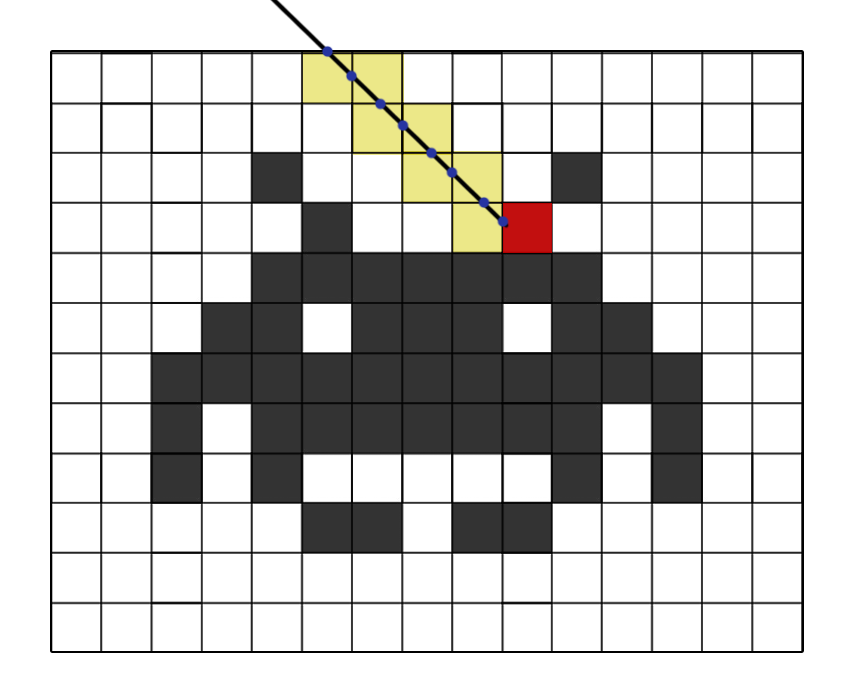
\includegraphics[width=90mm]{getVoxel.png}
	\caption{Vizualizácia fungovania algoritmu getVoxel}
	\label{invader}
\end{figure} 



\subsection{Štetec}
	Taktiež aj tento nástroj poskytuje dve funkcionality. Tou prvou je pridávanie voxelov na povrch objektu a tou druhou je zafarbovanie zakliknutých voxelov.
	Základom tohoto nástroja, ako aj mnohých nasledujúcich je opísaná funkcia na získavanie voxelov.
	Pri pridávaní voxelu sa získa kliknutý voxel a naň sa prilepí ďalší, zafarbený na natavenú farbu štetca. Pri zafarbovaní sa jednoducho zakliknutý voxel prefarbí podľa farby štetca. 
\subsection{Guma}
	Tento nástroj využíva funckiu získavania voxelov na ich mazanie. Pri zmazaní voxelu sa lokálne upravia okolité voxely, tak aby boli viditeľné. Teda sa im nastaví flag \textit{visible} na \textit{TRUE}.
\subsection{Kvapátko}
	Kvapátko je nástroj, ktorý už celé desaťročia mätie užívateľov svojím názvom. Slúži na získavanie farby z voxelu na kliknutie, preto bola aj pre tento nástroj potrebná funkcia na získavanie voxelu. 
\subsection{Výplň}
	Posledným nástrojom z rady implementovaných, ktorý používaja funkciu získavania voxelu pomocou lúča, je výplň. Tento nástroj zafarbí všetky voxely objektu, ktoré sú tranzitívne spojené so zakliknutým voxelom a zafarbí ich na farbu nastavenú v prostredí. To, že sú dva voxely spojené chápeme tak, že sú k sebe priamo susediace a zároveň sú rovnakej farby. Opísana procedúra priamo zachytáva algoritmus \textit{flood fill}, ktorý je len potrebné preniesť do priestoru.
\subsubsection{3D flood fill} 
	S veľmi pochabými úmyslami sme sa pustili do implementácie algoritmu rovno dvoma spôsobmi. \\
	Ako prvé sme zvolili rekurzívne riešenie a algoritmus prehľadávania do hĺbky. Funkciu bolo jednoduché implementovať, avšak už pri prvom testovaní sme narazili na veľký problém. Neuvedomili sme si, že pri veľkom počte voxelov sa funkcia vnára príliš hlboko do seba a teda nevyhnutne spôsobuje chybu pretečenia zásobníka
	
	Nefungujúcu funkciu bolo následne nutné prepísať tak, aby neobsahovala rekurziu. Tento problém sme vyriešili použitím radu a teda sme nahradili prehľadávanie do hĺbky, algoritmom prehľadávania do šírky.
	Naše riešenie teda vyzerá asi takto:
	
	\eject
	
	\begin{algorithmic}
		\Function{flood\_fill3D}{$indeces$}  
			\State $Visited \gets$ [ ]
			\State $Queue \gets [indeces]$
			\Repeat  
				\State $position \gets$ pop positon from $Queue$
				\If {$\NOT$($position$ in $Visited)$}
					\State Change color of voxel at $position$
					\ForAll{$position$ neighbours of same color}
						\State $Queue \gets Queue + [neighbour]$
					\EndFor
				\EndIf 
			\Until{$Queue$ is empty}
		\EndFunction \\
	\end{algorithmic} 
	
	{Finálne riešenie bolo ešte nutné pre urýchlenie upraviť tak, aby sme sa vyhli častému volaniu kopírovacích konštruktorov, použitím smerníkov.}
\subsection{Kamera}
	Tento nástroj je veľmi dôležitý pre užívateľa, aby sa rozumným spôsobom mohol orientovať v scéne. Ohnisko kamery je defaultne nastavené na stred celej scény, teda na bod $(0,0,0)$. Pri selekcii objektu pravým tlačidlom myši sa však ohnisko kamery zmení na stred označeného objektu.
	Kamera nám umožňuje orientáciu v scéne dvoma spôsobmi. Prvým je rotácia kamery okolo ohniska a druhým je približovanie sa alebo odďaľovanie od objektu, inak povedané zoom.
\subsection{Posun objektov}\label{moveTool}
	Označené objekty je možné posúvať na dragovaciu udalosť v troch rovinách. \\
	Kliknutie na objekt určí rovinu, v ktorej je možné objekt pohybovať podľa toho, na ktorú stenu užívateľ klikol. Okolo objektu sa následne zobrazí obdĺžnik, ktorý túto rovinu vizualizuje ako pomôcku pre užívateľa. Takéto riešenie je asi jediné svojho druhu, no napriek tomu ho považujeme za celkom jednoduché a intuitívne.


\section{Import/Export}\label{sec:io}
Modelovacie aplikácie akou je aj tá naša si vyžadujú import a export dát do a z programu. Rozhodli sme nájsť špecifikácie rôznych formátov voxelových súborov, ktoré už existujú, aby sme dosiahli čo najlepšiu variabilitu programu pri použití v praxi. Okrem ukladania dát do binárnych voxelových súborov je možné scénu exportovať do XML štruktúry alebo aj ako povrchový model vygenerovaný z voxelového.
\subsection{Polygónový model}
\subsubsection{Import}
Keďže všetky modely, ktoré sa nachádzajú v programe je možné uchovávať a zobrazovať iba v podobe voxelových objektov, import klasického povrchového modelu predstavuje nutnosť konverzie 3D meshu na voxely. Tento proces je tiež nazývaný \textit{voxelizácia}.
\eject
\subsubsection{Voxelizácia}
Vo všeobecnosti proces voxelizácie produkuje množinu hodnôt v pravidelnej trojrozmernej mriežke z objektov určených povrchovou reprezentáciou. Cieľom voxelizácie je vytvoriť voxelový objekt, ktorý je čo najbližšou možnou aproximáciou k originálnemu objektu. \cite{Voxelization}
Presnosť výsledku samozrejme závisí aj od rozmerov mriežky, ktoré si zvolíme. Kritickými miestami tohoto procesu môžu byť objekty s nulovou hrúbkou, alebo objekty s nekonvexnými dierami.

Riešenia opísané Georgom Passalisom \cite{Voxelization} využívajú možnosti GPU prostredníctvom funkcií OpenGL. Základná myšlienka spočíva v použití z-bufferov, vyprodukovaných povrchovými objektami, na voxelizáciu.
Algoritmus, ktorý prezentuje Karabassi potrebuje 3 páry z-bufferov, kde každá dvojica je určená pre jednu os. Kamera sa umiestni na všetkých 6 plôch pomyselného bounding boxu voxelizovaného objektu a s použitím ortogonálnej projekcie sa zapíšu dáta do bufferov. \cite{BufferVox}

Toto riešenie je pomerne jednoduché, avšak v istých prípadoch produkuje neželané výsledky. Ďalšia implementácia voxelizácie spomenutá v tomto článku rieši nedostatky tohoto algoritmu použítím komplikovaných shaderov, a preto sme sa rozhodli túto metódu nepoužiť a zvolili sme priamočiarejší prístup k problému.

Naše riešenie napasuje voxelizovaný objekt do mriežky s danými rozmermi a pre každú bunku mriežky určí, či sa jej stred nachádza v objekte alebo nie. Ak sa daný bod v objekte nachádza, pridáme voxel do objektu, ak sa nenachádza, tak nepridáme nič, respektíve pridáme nullovú hodnotu.
\eject
Približne takto vyzerá náš program: 

\begin{algorithmic}
	\State $\bullet$ Vytvor trojrozmernú mriežku \textit{M} s rozmermi $(width, height, depth)$
	\State $\bullet$ Naškáluj objekt \textit{O} do danej mriežky (tak aby sa objekt nedeformoval)
	\ForAll{$bunka \in M$}
		\If{ $bunka$ sa nachádza v $O$ }
			\State $\bullet$ Pridaj voxel do objektu.
		\Else
			\State $\bullet$ Pridaj $NULL$ do objektu.
		\EndIf
	\EndFor \\
\end{algorithmic} 

Takýto prístup je intuitívny a ľahko pochopiteľný aj pre laika. Rozhodujúcu úlohu v algoritme zohráva metóda zobrazená na obrázku \ref{ray}, ktorá determinuje, či sa bod nachádza v objekte alebo nie. Túto úlohu sme vyriešili tak, že sa z daného bodu vyšle lúč (polpriamka), a spočítajú sa priesečníky lúča s povrchom objektu. Ak ich počet je nepárny znamená to, že bod sa v objekte nachádza, inak sa v objekte nenachádza. Takto sa nám úloha posunula na ďalší podproblém zisťovania priesečníku polpriamky s polygónom. Keďže nájsť priesečník priamky s trojuholníkom je ľahšie ako s ľubovoľným polygónom, triangulizovali sme objekt už pri načítavaní zo súboru a potom sme mohli nájsť priesečník polpriamky s rovinou trojholníka a následne pomocou barycentrických súradníc sme rozhodli, či sa v ňom daný priesečník nachádza. 


Na obrázku \ref{ray} vidno fungovanie algoritmu na zistenie, či sa bod nachádza v objekte. Môžete vidieť dva príklady, kedy je lúč vyslaný z daného bodu na hor. V prvom prípade je nájdený párny počet priesečníkov, teda sa bod nenachádza v objekte a v druhom prípade ich je nájdených nepárny počet, teda sa bod v objekte nachádza.
\begin{figure}[h]
	\centering
	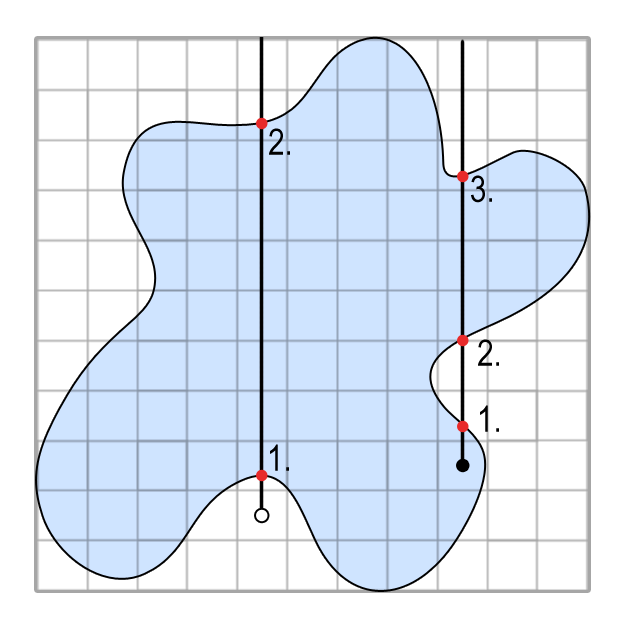
\includegraphics[width=0.6\textwidth]{ray.png}
	\caption{Vizualizácia algoritmu zisťovania, či sa bod náchádza v objekte}
	\label{ray}
\end{figure}


\subsubsection{Export}
Z každého voxelového objektu je možné extrahovať jeho povrchovú informáciu a vytvoriť z nej klasický 3D model.
Táto vlastnosť je užitočná napríklad pri postprocesingu, ak by sme napríklad chceli vytvoriť kvalitný render voxelových objektov.
Náš algoritmus prechádza všetky voxely v objekte, vypočíta pozíciu všetkých krajných 8 bodov voxelu a pre každý určí, či sa nachádza na povrchu objektu alebo nie. Následne tieto body pridá do poľa tak, aby sa v ňom nenachádzali duplicitne a do ďalšieho poľa si zapamätá poradie bodov, aby bolo možné danú viditeľnú stenu rekonštruovať.

\subsection{Bitmapa}
Do programu sme zahrnuli aj možnosť importovania bitmapy do prostredia. Spôsob, akým to robíme, je pomerne jednoduchý. Načítame si bitmapu zo súboru do pamäte a následne si vytvoríme voxelový objekt s hĺbkou 1 a šírkou a výškou rovnajúcimi sa rozmerom obrázka. Teraz nám stačí už len prejsť všetky body bitmapy a pridať voxel príslušnej farby do objektu. 

\subsection{Voxelové formáty}
Špecifikáciu bežne používaných voxelových formátov sme získali zo zdrojových kódov opensoruce programu \textit{binvox} \cite{binvox}. Vďaka tomu sa nám podarilo pridať do ponuky aplikácie pomerne veľké množstvo rôznych výstupných a vstupných formátov. 

\begin{multicols}{2}
Výstupné formáty:
\begin{itemize}
	\item Binvox
	\item RawVox
	\item Hips
	\item Mira
	\item Vt
	\item Vtk
\end{itemize}

Vstupné formáty:
\begin{itemize}
	\item Binvox
	\item Vox
	\item Mira
	\item Vt
	\item Vtk
\end{itemize}
\end{multicols}
Tieto formáty sa štruktúrou na seba dosť podobajú. Zaujímavým z nich je napríklad Binvox, ktorý používa RLE kódovanie na kompresiu dát a najjednoduchším z nich je RawVox, ktorý v sebe uchováva surové dáta tak, že na mieste voxelu ukladá $1$ a na mieste prázdneho miesta $0$.
Ich veľkou nevýhodou je, že nie je možné v nich ukladať viacej objektov naraz a taktiež neuchovávajú informáciu o farbe voxelov. Aby sme mohli ukladať celé scény pred začatím zapisovania dát do súboru, zlúčime všetky objekty v scéne a následne takto vzniknutý objekt uložíme.

\subsection{XML}
Keďže všetky známe formáty na ukladanie voxelov do súborov sú binárne a neumožňujú ukladanie farieb a ani celých scén s väčším množstvom objektov. Rozhodli sme sa ukladať scény do nami navrhnutej XML štruktúry. Takýto výstup je nielen viacej čitateľný, ale môžme si dovoliť uložiť akékoľvek informácie navyše, ktoré potrebujeme. Jeho nevýhodou oproti binárnym súborom je však jeho velkosť.
Import aj export XML sme implementovali prostredníctvom vyššie spomenutej knižnice \textit{pugixml}.
\eject
Takto vyzerá nami navrhnutá XML štruktúra:

\begin{framed}
\begin{lstlisting}
<?xml version="1.0" encoding="utf-8"?>
<cubo>
  <scene width="" height="" depth="">
    <positions>
      <position index="" x="" y="" z="" />
                    ...
    </positions>
    <objects>
      <object width="" height="" depth="" position="">
        <colors>
          <color index="" red="" green="" blue="" alpha="" />
                              ...
        </colors>
        <voxels sample="">
          <voxel i="" j="" k="" color="" />
                       ...
        </voxels>
      </object>
         ...
    </objects>
  </scene>
</cubo>
\end{lstlisting}

\end{framed}

\chapter{Výsledky}\label{chap:vyledky}
V tejto kapitole uvádzame merania výkonu aplikácie a taktiež niektoré vizuálne výsledky, ktoré sme získali na výstupe z aplikácie.

\section{Metodika merania}
Merania sme vykonávali na verzii programu skompilovanej v \textit{release} móde, od čoho sme si sľubovali lepšie výsledky. Merania FPS sme vykonali pomocou programu \textit{Fraps} \cite{fraps} a na merania času sme použili  zabudovanú funkciu \textit{clock()}, ktorá meria čas v milisekundách. Na odtestovanie voxelových súborov sme použili program \textit{viewvox} \cite{viewvox}, ktorý je spustiteľný cez konzolu, avšak nedokáže otvoriť všetky implementované súborové formáty.

Testy prebiehali pod 32-bitovým operačným systémom Microsoft Windows 7 Ultimate. Testovací hardvér bol AMD Turion X2 Dual-Core Mobile RM-72 2.1 GHz, 3GB DDR2 pamäte, zabudovaná grafická karta ATI Mobility Radeon HD 3400 Series 512MB. Na hardvéri boli nainštalované grafické ovládače Catalyst 8.97.100.7 16-XI-12 podporujúce OpenGL 3.3.

\section{Rendering}

Rýchlosť renderovania je závislá od počtu voxelov v scéne a tvaru samotného objektu. Ucelené tvary dosahujú lepšie výsledky, ako tvary s veľkým množstvom dier vo vnútri objektu, keďže program je nastavený tak, že skrýva voxely obkolesené zo všetkých strán.
V tabuľke \ref{tab:voxels} je zobrazený počet voxelov pre rôzne objekty a rôzne rozmery. Na objektoch s týmito rozmermi sme následne vykonali testy FPS. Tabuľka \ref{tab:fps} zobrazuje  výsledky testovania pre dané objekty. \\

\begin{table}[hp]
  \centering
  \begin{tabular}{|l|l|l|l|l|l|}
  \hline
  Tvar \ Rozmery & 
  \begin{math}16^3\end{math} & 
  \begin{math}32^3\end{math} & 
  \begin{math}64^3\end{math} & 
  \begin{math}128^3\end{math} \\
  \hline
  Kocka & 4096 & 32 768 & 262 144 & 2 097 152\\
  \hline
  Guľa & 2176 & 17 256 & 137 376 & 1 099 136\\
  \hline
  Kužeľ & 1108 & 8680 & 68 672 & 549 760\\
  \hline
  Náhodne generovaný objekt & 2058 & 16 490 & 131 072 & --- \\ 
  \hline
  \end{tabular}
  \caption{Tabuľka počtov voxelov na objekt}
  \label{tab:voxels}
\end{table}


\begin{table}[!h]
  \centering
  \begin{tabular}{|l|l|l|l|l|l|}
  \hline
  Tvar \ Rozmery & 
  \begin{math}16^3\end{math} & 
  \begin{math}32^3\end{math} & 
  \begin{math}64^3\end{math} & 
  \begin{math}128^3\end{math} \\
  \hline
  Kocka & 62 FPS & 19 FPS & 5 FPS & 1 FPS \\
  \hline
  Guľa & 105 FPS & 35 FPS & 9 FPS & 2 FPS \\
  \hline
  Kužeľ & 110 FPS & 40 FPS & 11 FPS & 3 FPS \\
  \hline
  Náhodne generovaný objekt & 48 FPS & 7 FPS & 1 FPS & --- \\ 
  \hline
  \end{tabular}
  \caption{Rýchlosti renderovania objektov namerané v FPS}
  \label{tab:fps}
\end{table}

Na obrázku \ref{ballRender} možno vidieť vyrenderovanú guľu o rozmeroch $128^3$ voxelov a počet framov za sekundu nameraných programom Fraps.

\begin{figure}[ht!]
	\centering
	\includegraphics[width=0.6\textwidth]{ballRender.png}
	\caption[Vyrenderovaná guľa]{Vyrenderovaná guľa zložená z 1 099 136 voxelov}
	\label{ballRender}
\end{figure}


\section{Voxelizácia}
Vybrali sme niekoľko známych povrchových modelov s rôznym počtom polygónov respektíve trojuholníkov, ktoré sme voxelizovali do mriežky rôznych rozmerov. Počas voxelizácie sme testovali čas, ktorý uplynie od začiatku funkcie voxelizácie po jej koniec. Nezapočítavali sme teda časový úsek, ktorý ubehne počas načítania polygónových modelov do pamäte. 

Taktiež sme vizuálne kontrolovali tvar výsledného voxelového objektu. V tabuľke \ref{tab:voxelization} sú zobrazené namerané údaje pre konkrétny model a rozmery. Celkovo voxelizácia dosahovala uspokojivé výsledky.

\begin{table}[!h]
  \centering
  \begin{tabular}{|l|l|l|l|l|}
  \hline
  Objekt(počet trojuholníkov) \ Rozmer & 
  \begin{math}16\end{math} & 
  \begin{math}32\end{math} & 
  \begin{math}64\end{math} & 
  \begin{math}128\end{math} \\
  \hline
  Suzanne (968) & 0.022 s & 0.125 s & 0.92 s & 6.88 s\\
  \hline
  Teapot (6321) & 0.078 s & 0.421 s & 2.418 s & 16.24 s\\
  \hline
  Pumpkin (10 000) & 0.123 s & 0.577 s & 3.074 s & 18.486 s\\
  \hline
  Standford bunny (69 666) & 1.17 s & 5.678 s & 30.467 s & 184.76 s \\ 
  \hline
  \end{tabular}
  \caption{Rýchlosti voxelizácie rôznych modelov}
  \label{tab:voxelization}
\end{table}


Na obrázku \ref{bunny} je vidno výsledky voxelizácie pre model \textit{Standford bunny} s 69666 trojuholníkmi v rozmeroch $32^3, 64^3 a 128^3$ voxelov.

\begin{figure}[ht!]
	\centering
	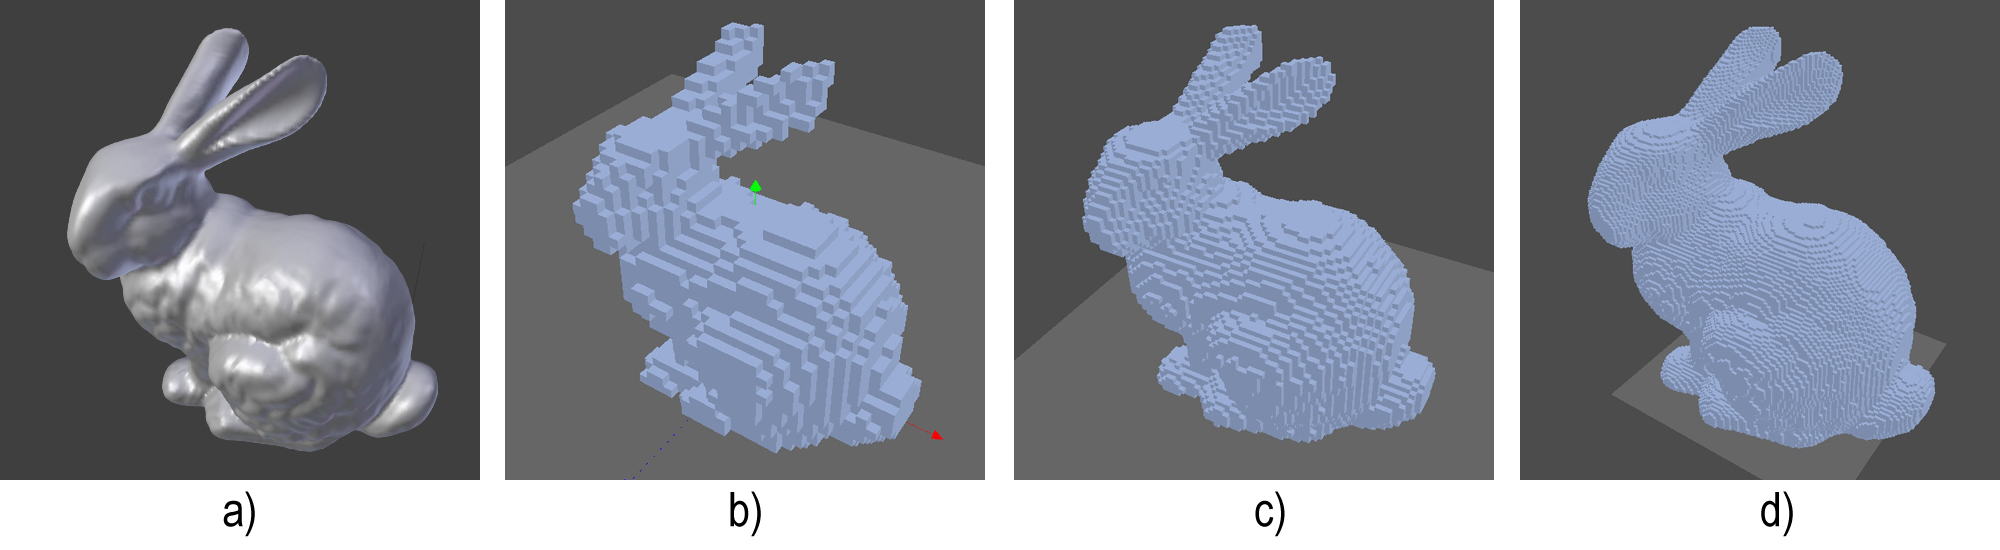
\includegraphics[width=1.0\textwidth]{bunny.jpg}
	\caption[Výsledky voxelizácie]{Výsledky voxelizácie. a) Originálny polygónový objekt b) $32^3$ c) $64^3$ d) $128^3$}
	\label{bunny}
\end{figure}

\section{Voxelové objekty}
Ako bolo spomenuté v kapitole \ref{chap:implementacia}, implementovali sme 5 základných voxelových tvarov: kváder, elipsoid, valec, ihlan a kužeľ. Výsledky implementácie môžete vidieť na obrázku \ref{shapes}. Na tomto obrázku vidno objekty v rozmeroch 20x20x20 voxelov, avšak je možné ich vytvoriť v ľubovoľných rozmeroch od 1 po 50. Aspoň takéto obmedzenia ponúka nami vytvorený interface na tvorbu voxelových tvarov.


Taktiež sme nad objektami implementovali boolovské operácie, ktoré v programe dosahovali očakávané výsledky ako je možné vidieť na obrázku \ref{bools}.


\begin{figure}[!h]
	\centering
	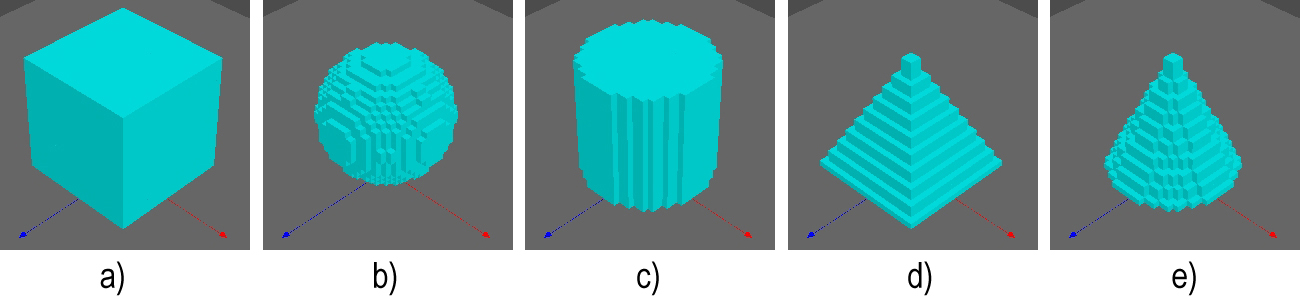
\includegraphics[width=1.0\textwidth]{shapes.jpg}
	\caption[Základné objekty]{Základné tvary. a) kocka(kváder) b) guľa(elipsoid) c) valec d) ihlan e) kužeľ }
	\label{shapes}
\end{figure}

\begin{figure}[!h]
	\centering
	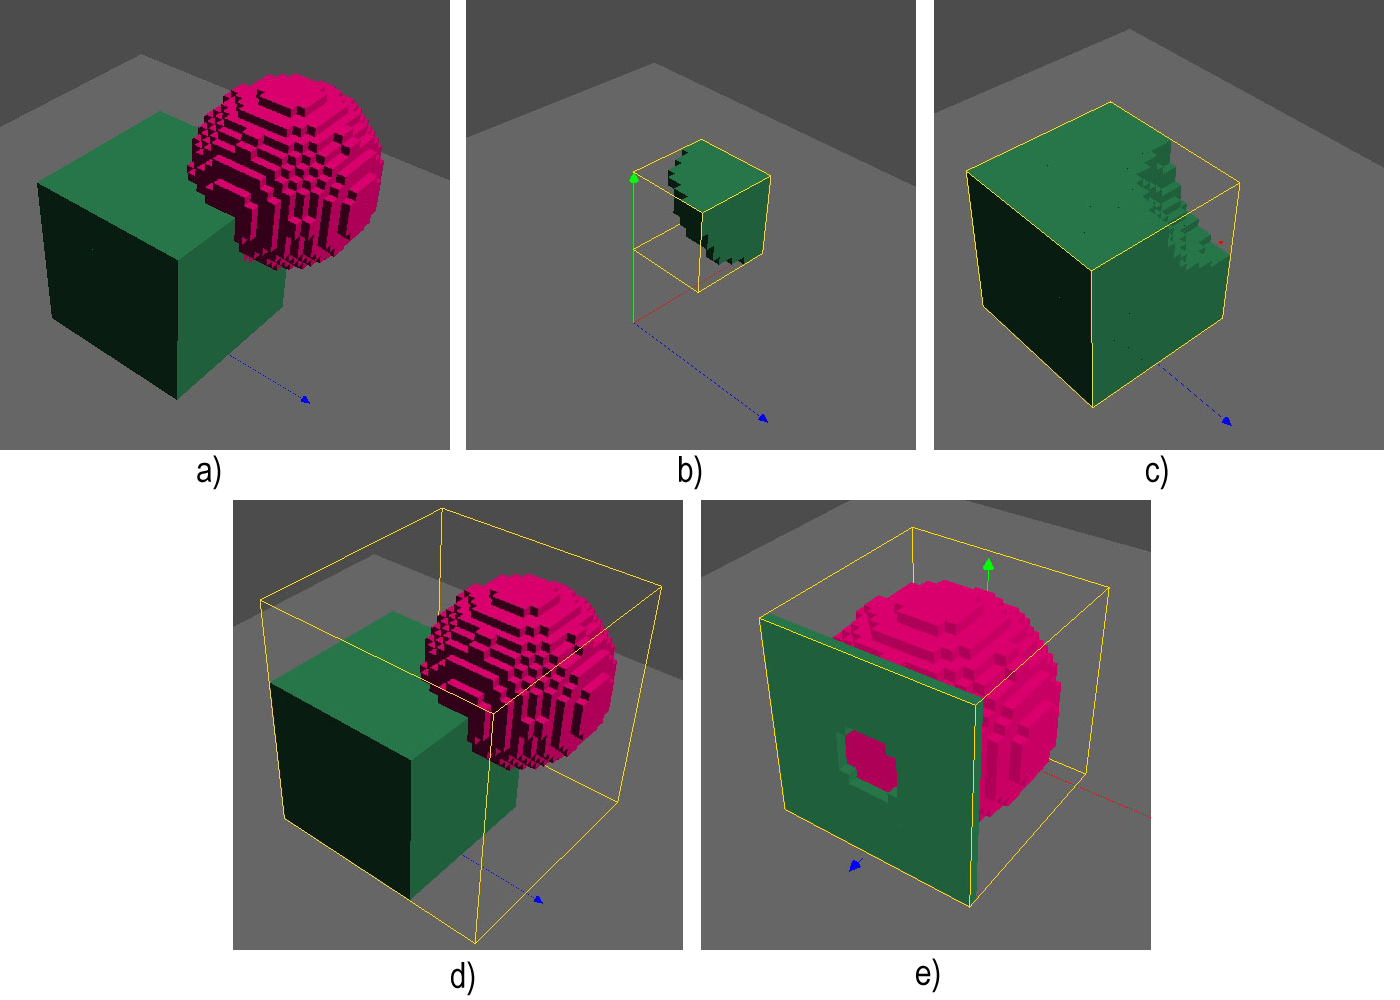
\includegraphics[width=1.0\textwidth]{bools.png}
	\caption[Booleanovské operácie]{Výsledok booleanovských operácií. a) Originálne objekty b) AND c) NOT d) OR e) XOR (nevznikol z objektov na obrazku a) )}
	\label{bools}
\end{figure}

\section{Nástroje}
Získavanie voxelov z objektu na kliknutie je dostatočne rýchle a teda základné nástroje, ktoré využívajú túto funkciu, ako napríklad \textit{štetec}, \textit{guma}, \textit{kvapkátko} a podobne, dosahujú želané výsledky a nestretli sme sa so žiadnymi závažnejšími problémami pri ich navrhovaní a ani používaní.

Zaujímavejším z nástrojov je napríklad nástroj \textit{výplň}, ktorého fungovanie je zložitejšie a časovo náročnejšie, keďže využíva algoritmus prehľadávania do šírky a teda v mnohých prípadoch prechádza cez všetky voxely objektu. Tento nástroj sme po prvotnom testovaní museli optimalizovať s použitím smerníkov, a tak sme dosiahli niekoľkonásobne väčšiu rýchlosť, keďže sme sa vyhli zbytočnému volaniu kopírovacích konštruktorov. 
 
Taktiež problémovými boli modifikačné nástroje s výnimkou translácie. V prípade škálovania a rotácie bolo potrebné vyriešiť vznikajúce diery, čo sa nám podarilo na základe spomenutých algoritmov v kapitole \ref{chap:implementacia} \textit{Implementácia} v sekcii \ref{voxelObjects} \textit{Voxelové objekty}. Výsledky našej implementácie týchto postupov môžete vidieť na obrázku \ref{modif}.
\begin{figure}[ht!]
	\centering
	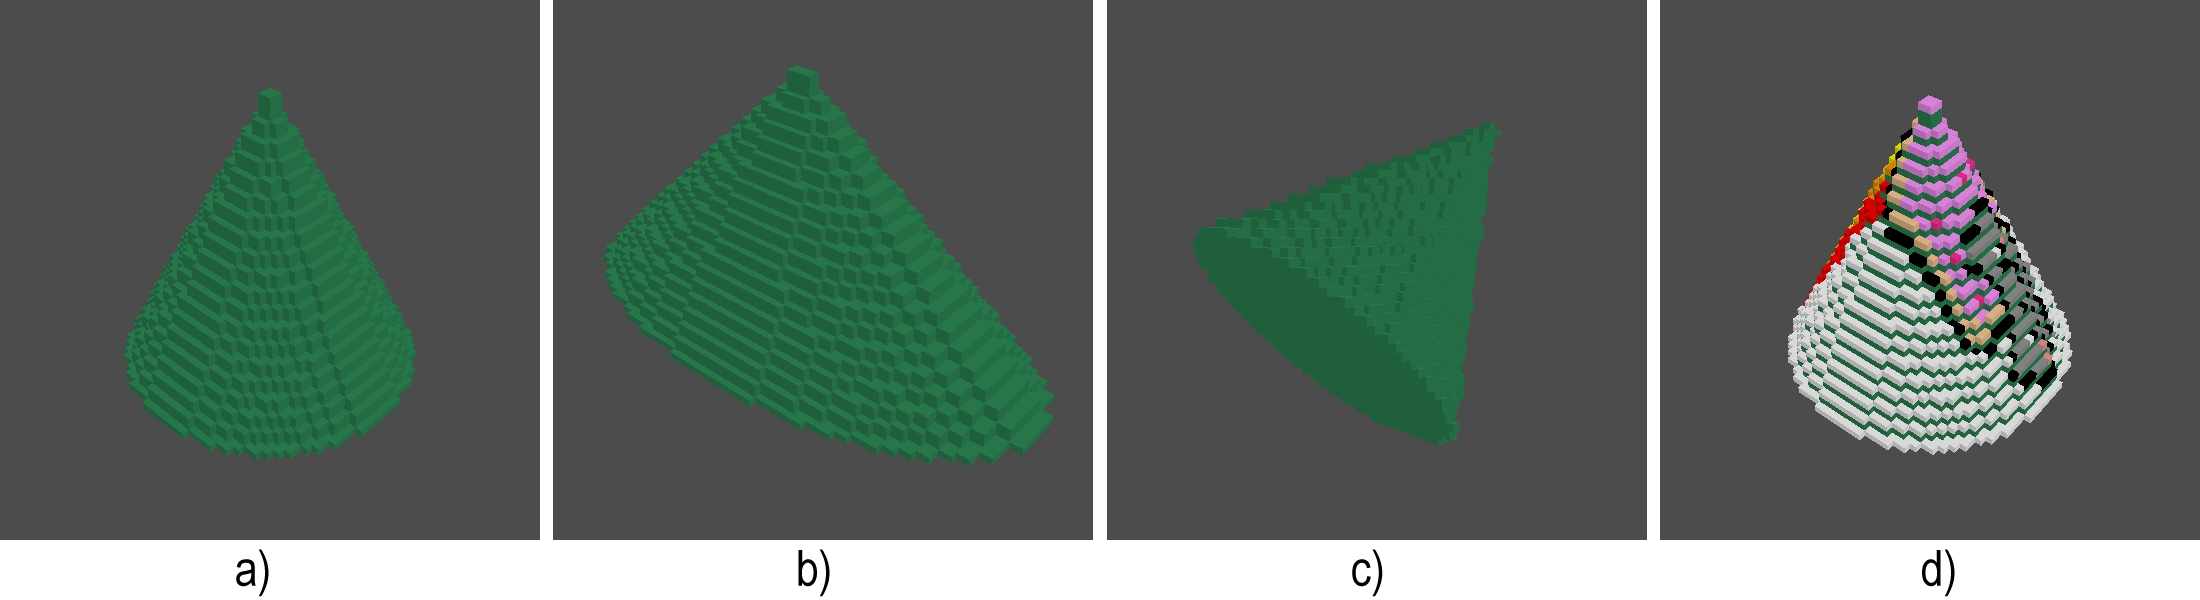
\includegraphics[width=1.0\textwidth]{modif.jpg}
	\caption[Transformácie obejktov]{Transformácie obejktov a textúrovanie. a) Pôvodný objekt  b) Naškálovaný objekt na dvojnásobnú šírku  c) Zrotovaný objekt o $45\,^{\circ}$ okolo osi $x$  d) Objekt s namapovanou textúrou}
	\label{modif}
\end{figure}

\section{Import/Export}
Testovanie importu a exportu voxelových súborov sme realizovali prostredníctvom programu na zobrazovanie voxelových objektov \textit{viewvox} a programu na voxelizáciu 3D modelov \textit{binvox} \cite{binvox}. Oba programy nepodporujú všetky nami implementované súborové formáty, preto bolo môžné vyskúšať ukladanie scény do formátov: .binvox, .mira a loadovanie súborov vygenerovaných programom binvox: .binvox, .mira, .vtk. 

Ako možno vidieť na obrázku \ref{io}, program viewvox pri zobrazovaní naškáluje objekt na rozmery $1\times1\times1$, čo spôsobuje deformáciu objektov, ktoré nemajú totožné všetky tri dimenzie. Ďalším rozdielom pri zobrazovaní je umiestnenie osí \textit{z} a \textit{y}, ktoré sú v našom prípade vymenené.

Pomocou programu binvox sme voxelizovali trojrozmerný polygónový objekt na voxelový o rozmeroch $64^3$ a uložili vo vyššie spomenutých formátoch. Takéto súbory sme sa potom snažili načítať do nášho prostredia. Prvý pokus nebol úspešný, ale po malých úpravách kódu sa nám súbory podarilo korektne spracovať a voxelové objekty načítať s vymenenou osou \textit{z} podobne ako pri programe viewvox. Ako bolo spomenuté v kapitole \ref{chap:implementacia} v sekcii \ref{sec:io} a ako možno vidieť na obrázku \ref{io} tieto formáty neumožňujú ukladanie farieb, a tak sa zobrazujú v defaultnej bielej farbe. 

Uskutočnili sme aj testy exportu a importu pre XML štruktúru. Výsledky boli očakávané a ničím zaujímavé, a preto ich tu ani neuvádzame.

\begin{figure}[!h]
	\centering
	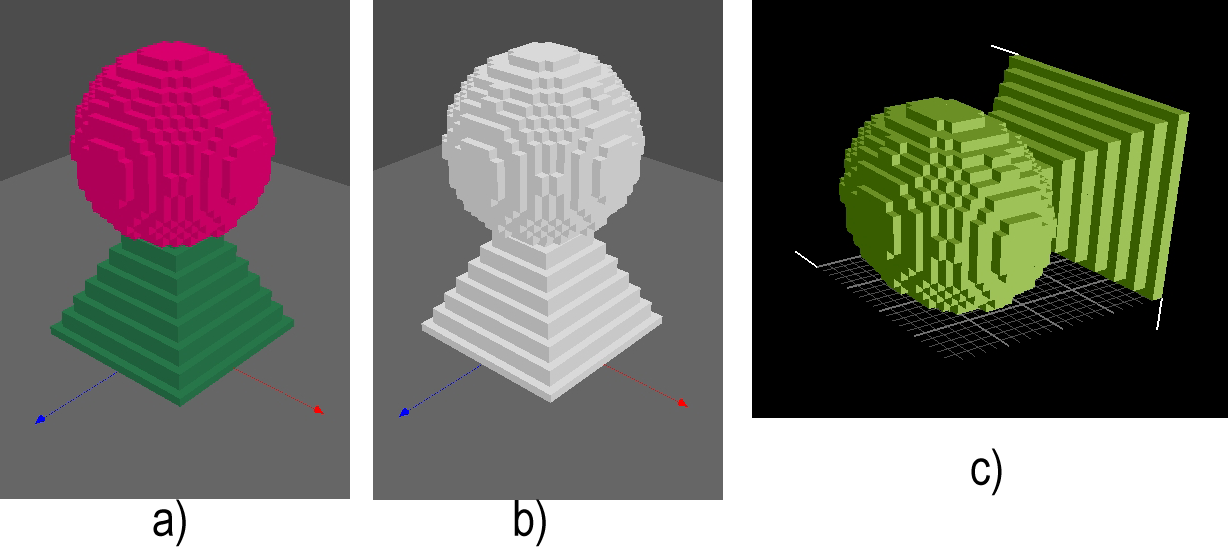
\includegraphics[width=0.8\textwidth]{export.png}
	\caption[Test exportu]{Výsledky testovania exportu do binárnych súborov. a) Exportovaný objekt b) Načítaný objekt v našom prostredí c) Načítaný objekt v programe viewvox}
	\label{io}
\end{figure}
\eject

Okrem importu meshu, teda voxelizácie, ktorej výsledky sme vyhodnotili vyššie, je možné do programu importovať rôzne obrázkové súbory.
 
Import bitmapy do prostredia bol taktiež zaujímavý. Podarilo sa nám vložiť akýkoľvek obrázkový formát, ktorý je schopná otvoriť knižnica DevIL, s výnimkou formátov, ktoré majú indexované farby ako napríklad gif. Na obrázku \ref{obr:cat} možno vidieť bitmapu mačky vo formáte PNG s transparentnými pixelmi (na obrázku ich vidno ako šedé) o rozmeroch $50\times50$ pixelov a objekt, ktorý vznikol importovaním tohoto obrázka do programu. Program zachováva transparenciu pixelov, ktoré majú hodnotu \textit{alpha} nulovú.

\begin{figure}[!h]
	\centering
	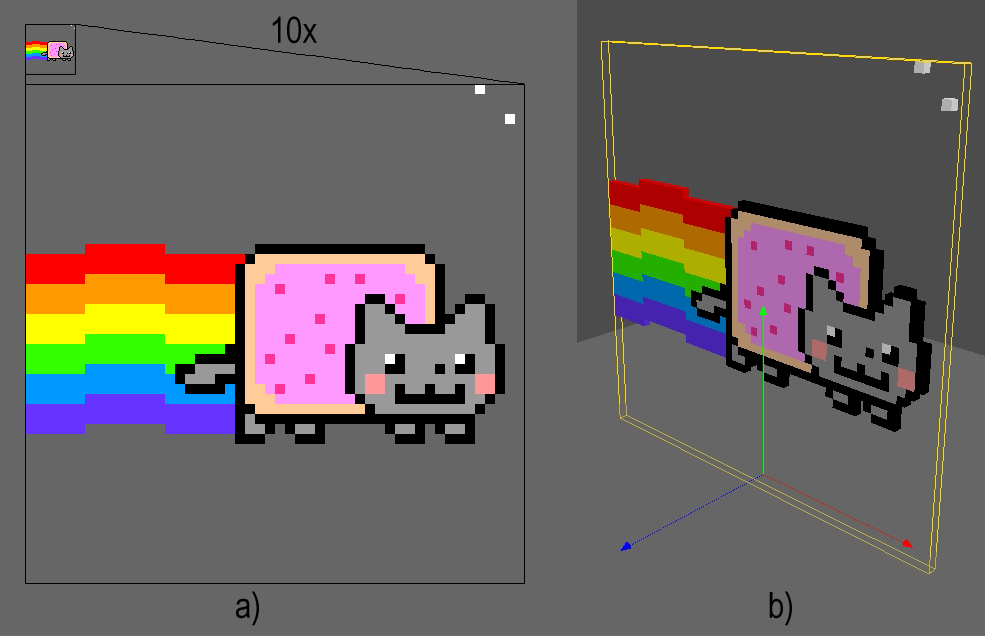
\includegraphics[width=0.8\textwidth]{cat.png}
	\caption[Import bitmapy]{Výsledok importu bitmapy. a) 10 násobne zväčšená bitmapa mačky b) importovaná bitmapa do prostredia}
	\label{obr:cat}
\end{figure}

\section{Užívateľské prostredie}
Pri tvorbe užívateľského prostredia sme kládli dôraz na vytvorenie čo najväčšieho pracovného priestoru. Výsledkom je, že najrozmernejšia časť okna aplikácie zaberá takzvané plátno, na ktoré je premietaná voxelová scéna. 

V ľavom paneli sa nachádzajú dve série ikoniek predelené oddeľovačom, z ktorých prvá sú základné editačné nástroje a druhá séria sú základné tvary, ktoré možno do prostredia vložiť. 

Ďalej sa tu nachádzajú ešte dve horizontálne lišty zarovnané na vrchný okraj okna. V jednej sa nachádzajú štyri ikonky, ktoré slúžia na booleanovské operácie nad objektami a druhá lišta obsahuje zvyšnú funkcionalitu programu, teda import a export, možnosť prepínania zobrazenia podlahy, osí, tieňovania a podobne a taktiež možnosť transformácie označených objektov.

Na obrázku \ref{ui} možno vidieť výsledné prostredie nášho editora, tak ako sme ho opísali v tejto sekcii.\\
\begin{figure}[!h]
	\centering
	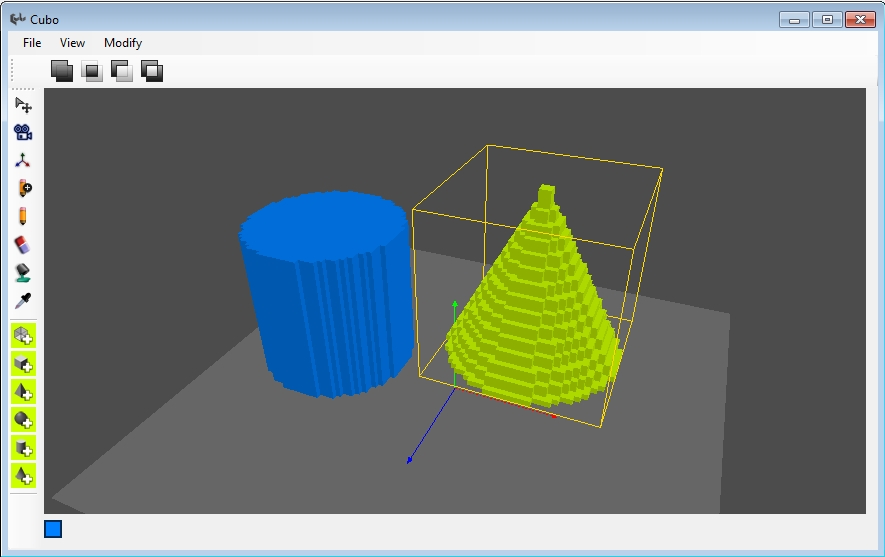
\includegraphics[width=1.0\textwidth]{UI.jpg}
	\caption[Užívateľské prostredie]{Screenshot z programu \textit{Cubo}}
	%\vspace*{3in}
	\label{ui}
\end{figure}
\clearpage
\begin{Huge}
\textbf{Záver} \\
\end{Huge}

V práci sme v stručnosti opísali základné poznatky z objemovej grafiky a dôležitosť nástroja na manipuláciu s voxelmi. Zadefinovali sme pojem \textit{voxel} a preskúmali sme výhody a nevýhody tohto elementu i v komerčnej sfére.

Uviedli sme malú vzorku existujúcich voxelových editorov a opísali sme výhody a nevýhody, ktorými sme sa inšpirovali, jednotlivo pre každý program.
Nadobudnuté poznatky sme ďalej aplikovali pri implementácii samotného voxelového editora.

Výsledkom práce je teda plne funkčný program s možnosťou vytvoriť takmer ľubovoľný voxelový objekt alebo scénu s obmedzením na rozmery. Vytvorená aplikácia ponúka uspkojivé množstvo modelovacích respektíve kresliacich nástrojov a taktiež možnosť importovať a exportovať scénu do XML, WaveFront(.obj) alebo aj rôznych binárnych voxelových formátov. V práci sme tiež opísali a implementovali algoritmus voxelizácie uzavretých polygónových objektov slúžiaci na import modelov do scény. \\

\textbf{Budúca práca} \\

Prakticky je možné prerobiť akúkoľvek funkciu nad rastrami, aby pracovala nad voxelmi, a presne tam vidíme ďalšiu možnosť vývoja aplikácie. Vo všeobecnosti je ďalší postup obmedzený iba našou fantáziou a časom, a preto spomenieme iba pár majoritných vylepšení. 

V prvom rade by bolo dôležité umožniť do prostredia vkladať a zobrazovať väčšie objemy dát. V momentálnom stave môžu mať objekty, bez vplyvu na rýchlosť, rozmery v ráde desiatok. Takýto stav je však nedostačujúci ale pri voxelových editoroch celkom bežný. Budúca snaha by bola optimalizovať uchovávanie dát a rendering, aby bolo možné vytvárať objekty v ráde stoviek až tisícok ako to je pri bežných rastrových nástrojoch.

Kedže sme implementovali iba jednoduché planárne mapovanie textúry na objekt, bolo by zaujímavé vytvoriť zložitejšie spôsoby textúrovania objektov s rôznymi nastaveniami.

K lepšiemu ovládaniu nástroja a obzvlášť k lepšiemu manipulovaniu s obsahom objektov by dopomohla funkcionalita kreslenia po vrstvách. Takto by bolo možné sa postupne posúvať po vrstvách objektu a vyplňovať bunky príslušnou farbou, čím by sa značne uľahčila práca.

Ďalším dôležitým chýbajúcim prvkom v aplikácii je možnosť vyrenderovania objektu do obrázka. Toto by si vyžadovalo komplikovanejší prístup a použitie renderovacích algoritmov v diskrétnom priestore, ako je napríklad diskrétny raytracing, ktorý opísal Ronie Yagel \cite{RayTracing}.
Okrem statického renderovania, by bolo veľmi zaujímvé vyrenderovať voxelovú animáciu, čo by vyžadovalo aj príslušné nástroje na správu framov, časovania, pohybu voxelov a podobne.



\bibliographystyle{alpha}
\raggedright
\bibliography{literatura}


\end{document}
